% la-08-bayes.tex

\documentclass[xcolor=dvipsnames]{beamer}
\usepackage{tikz}
\usepackage{teachbeamer}

\title{Axioms and Theorems of Probability}
\subtitle{{\CourseNumber}, BCIT}

\author{\CourseName}

\date{November 13, 2018}

\begin{document}

\begin{frame}
  \titlepage
\end{frame}

\begin{frame}
  \frametitle{Introductory Concepts in Statistics I}
  \begin{itemize}
  \item<1-> A \alert{population} is the complete collection of all
    measurements or data that are being considered.
  \item<2-> A \alert{census} is the collection of data from every
    member of the population.
  \item<3-> A \alert{sample} is a subcollection of members selected
    from a population.
  \end{itemize}
\end{frame}

\begin{frame}
  \frametitle{Introductory Concepts in Statistics II}
  \begin{itemize}
  \item<1-> A \alert{voluntary response sample} or
    \alert{self-selected sample} is one in which the respondents
    themselves decide whether to be included.
  \item<2-> A \alert{random sample} is one in which each member has
    the same probability of being selected.
  \item<3-> A \alert{stratified random sample} is one in which random
    samples from subgroups are drawn and proportionally combined to
    form the complete sample.
  \end{itemize}
\end{frame}

\begin{frame}
  \frametitle{Introductory Concepts in Statistics III}
  \begin{itemize}
  \item<1-> A \alert{parameter} is a numerical measurement describing
    some characteristic of the population.
  \item<2-> A \alert{statistic} is a numerical measurement describing
    some characteristic of a sample.
  \end{itemize}
\end{frame}

\begin{frame}
  \frametitle{Introductory Concepts in Statistics IV}
  \begin{itemize}
  \item<1-> \alert{Quantitative} (or \alert{numerical}) data consist
    of numbers representing counts or measurements.
  \item<2-> \alert{Categorical} (or \alert{qualitative}) data consist
    of names or labels that are not numbers representing counts or
    measurements.
  \end{itemize}
\end{frame}

\begin{frame}
  \frametitle{Introductory Concepts in Statistics V}
  \begin{itemize}
  \item<1-> \alert{Discrete} data result when the data values are
    quantitative and the number of values is finite or countable.
  \item<2-> \alert{Continuous} data result when the data values are
    quantitative and the number of values is infinite and not
    countable.
  \end{itemize}
Here is an example for infinite discrete outcomes (this is rare). Roll
a die until you roll a six. There are infinitely many ways to do this,
but the data is not continuous.
\end{frame}

\begin{frame}
  \frametitle{Introductory Concepts in Statistics VI}
  \begin{itemize}
  \item<1-> \alert{Blinding} is when the subject doesn't know whether
    they are receiving a treatment or a placebo.
  \item<2-> The \alert{placebo effect} occurs when an untreated
    subject reports an improvement in symptoms because of their
    participation in the study.
  \item<3-> An experiment is \alert{double-blind} when it is blind and
    the experimenter also doesn't know whether they are applying a
    treatment or a placebo.
  \end{itemize}
\end{frame}

\begin{frame}
  \frametitle{Correlation Does Not Imply Causation}
\alert{Confounding} occurs in an experiment when the investigators are
not abloe to distinguish among the effects of different factors.
\begin{figure}[h]
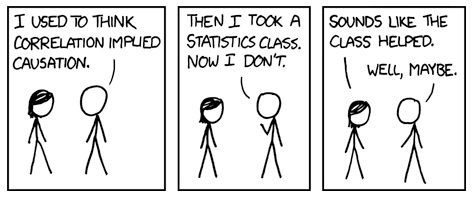
\includegraphics[scale=.3]{./diagrams/xkcd-causation-correlation.png}
\end{figure}
Examples: 
\begin{enumerate}
\item<1-> astrological sign and IQ in elementary school
\item<2-> soft drinks and obesity
\item<3-> birth control pills and thrombosis
\end{enumerate}
\end{frame}

\begin{frame}
  \frametitle{Modes of Data Presentation}
The three modes of data presentation.
\begin{itemize}
\item textual
\item tabular
\item graphical
\end{itemize}
\end{frame}

\begin{frame}
  \frametitle{Textual}
Example for textual data presentation.
\begin{block}{Philippine Stock Market}
The Philippine Stock Exchange composite index lost 7.19 points to
2,099.12 after trading between 2,095.30 and 2,108.47. Volume was 1.29
billion shares worth 903.15 million pesos (16.7 million dollars). The
broader all share index gained 5.21 points to 1,221.34. (From: Freeman
dated March 17, 2005)
\end{block}
\end{frame}

\begin{frame}
  \frametitle{Types of Graphs}
Four types of graphs.
\begin{itemize}
\item Line plot
\item Pie chart
\item Bar plot
\item Multi-bar graph
\item Histogram
\end{itemize}
\end{frame}

\begin{frame}
  \frametitle{Line Plot}
Usually suitable for data on a timeline. Here is an example. Rainy
days in Vancouver.

\begin{tabular}{|l|r|r|r|r|}\hline
  & Q1 & Q2 & Q3 & Q4 \\ \hline
2012 & 55 & 43 & 13 & 65 \\ \hline
2013 & 53 & 41 & 27 & 35 \\ \hline
2014 & 45 & 38 & 18 & 54 \\ \hline
2015 & 49 & 19 & 25 & 53 \\ \hline
2016 & 61 & 28 & 27 & 69 \\ \hline
\end{tabular}
\end{frame}

\begin{frame}
  \frametitle{Data for Line Plot Example}
Here is the file \texttt{fs01.csv}. On a Windows computer, open the
program called Notepad and paste the data into it. Then save as
\texttt{fs01.csv}. You can then open this file in R Studio, for
example (but also in other statistical software, such as minitab or
excel). 
\begin{alltt}
\tiny
year,quarter,dor\newline
2012,Q1,55\newline
2012,Q2,43\newline
2012,Q3,13\newline
2012,Q4,65\newline
2013,Q1,53\newline
2013,Q2,41\newline
2013,Q3,27\newline
2013,Q4,35\newline
2014,Q1,45\newline
2014,Q2,38\newline
2014,Q3,18\newline
2014,Q4,54\newline
2015,Q1,49\newline
2015,Q2,19\newline
2015,Q3,25\newline
2015,Q4,53\newline
2016,Q1,61\newline
2016,Q2,28\newline
2016,Q3,27\newline
2016,Q4,69
\end{alltt}
\end{frame}

% \begin{frame}
%   \frametitle{Line Plot Example By Quarter}
% In R Statistics, use the file \texttt{fs01.csv} and the following
% code.
% \begin{alltt}
% \small
% a<-read.table("fs01.csv",sep=",",header=TRUE)\newline
% b1<-subset(a,quarter=="Q1",select=c(dor))\newline
% b2<-subset(a,quarter=="Q2",select=c(dor))\newline
% b3<-subset(a,quarter=="Q3",select=c(dor))\newline
% b4<-subset(a,quarter=="Q4",select=c(dor))\newline
% ylima<-min(a[[3]])-3\newline
% ylimb<-max(a[[3]])+3\newline
% plot(b1[[1]],type="o",ylim=c(ylima,ylimb),col="blue")\newline
% lines(b2[[1]],type="o",col="red")\newline
% lines(b3[[1]],type="o",col="green")\newline
% lines(b4[[1]],type="o",col="yellow")
% \end{alltt}
% \end{frame}

% \begin{frame}
%   \frametitle{Line Plot Example By Quarter}
% \begin{figure}[h]
% 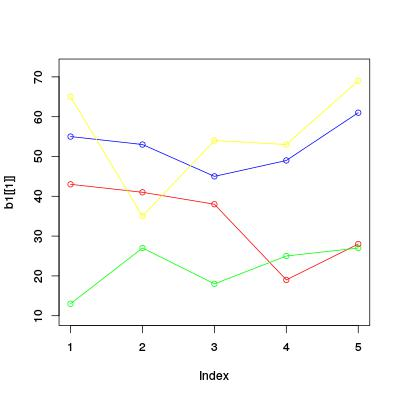
\includegraphics[scale=.6]{./diagrams/lineplot1.jpg}
% \end{figure}
% \end{frame}

\begin{frame}
  \frametitle{Line Plot Example By Year}
In R Statistics, use the file \texttt{fs01.csv} and the following
code.
\begin{alltt}
\small
a<-read.table("fs01.csv",sep=",",header=TRUE)\newline
c1<-subset(a,year=="2012",select=c(dor))\newline
c2<-subset(a,year=="2013",select=c(dor))\newline
c3<-subset(a,year=="2014",select=c(dor))\newline
c4<-subset(a,year=="2015",select=c(dor))\newline
c5<-subset(a,year=="2016",select=c(dor))\newline
ylima<-min(a[[3]])-3\newline
ylimb<-max(a[[3]])+3\newline
plot(c1[[1]],type="o",ylim=c(ylima,ylimb),col="blue")\newline
lines(c2[[1]],type="o",ylim=c(ylima,ylimb),col="red")\newline
lines(c3[[1]],type="o",ylim=c(ylima,ylimb),col="green")\newline
lines(c4[[1]],type="o",ylim=c(ylima,ylimb),col="yellow")\newline
lines(c5[[1]],type="o",ylim=c(ylima,ylimb),col="orange")
\end{alltt}
\end{frame}

\begin{frame}
  \frametitle{Line Plot Example By Year}
\begin{figure}[h]
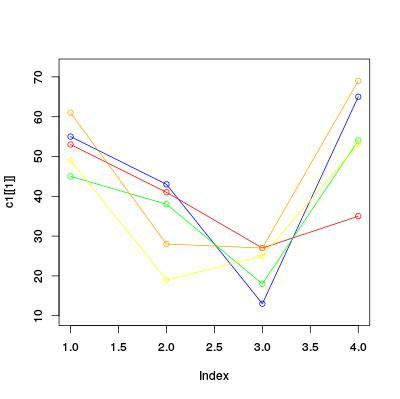
\includegraphics[scale=.6]{./diagrams/lineplot2.jpg}
\end{figure}
\end{frame}

\begin{frame}
  \frametitle{Pie Chart}
Pie charts are often used for tabular representations of categorical
data. Consider the following data set \texttt{fs02.csv} and the
corresponding chart on the next slide.
\begin{alltt}
\small
party,votes\newline
LIB,6943276\newline
CON,5613614\newline
NDP,3470350\newline
BQU,821144\newline
GRN,602944
\end{alltt}
\end{frame}

\begin{frame}
  \frametitle{Pie Chart Graph}
We are using the following R commands: 
\begin{alltt}
\small
d<-read.table("fs02.csv",sep=",",header=TRUE)\newline
pie(d[[2]],label=d[[1]])
\end{alltt}

However, pie charts are not recommended for visualizing statistical
data. Bar plots make differences between data points more clear.
\begin{figure}[h]
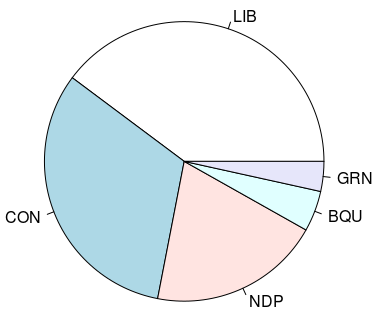
\includegraphics[scale=.5]{./diagrams/pie.png}
\end{figure}
\end{frame}

\begin{frame}
  \frametitle{Bar Plot Graph}
\begin{figure}[h]
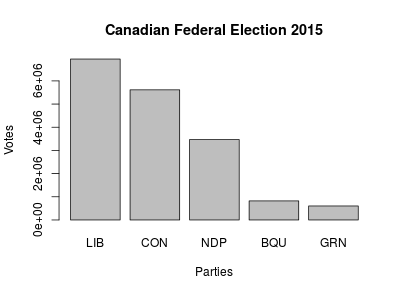
\includegraphics[scale=.5]{./diagrams/barplot.png}
\end{figure}
We have used the following R command: 
\begin{alltt}
\small
barplot(d[[2]], main="Canadian Federal Election 2015",\newline
xlab="Parties",ylab="Votes",names.arg=d[[1]])
\end{alltt}
\end{frame}

\begin{frame}
  \frametitle{Multi-Bar Graph}
Use the following R commands for a multi-bar graph of tabular data: 
\begin{alltt}
\small
e<-read.table("fs03.csv",sep=",",header=TRUE)\newline
barplot(as.matrix(e),beside=TRUE,col=rainbow(4))
\end{alltt}
Here is how to organize the data in the file \texttt{fs03.csv} for these commands:
\begin{alltt}
\small
y2012,y2013,y2014,y2015,y2016\newline
55,53,45,49,61\newline
43,41,38,19,28\newline
13,27,18,25,27\newline
65,35,54,53,69
\end{alltt}
These are the rainy days in Vancouver as in \texttt{fs01.csv}, but
organized in tabular form.
\end{frame}

\begin{frame}
  \frametitle{Multi-Bar Graph}
\begin{figure}[h]
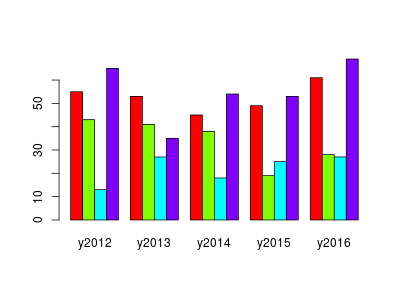
\includegraphics[scale=.8]{./diagrams/mbg.png}
\end{figure}
\end{frame}

\begin{frame}
  \frametitle{Histogram}
We use histograms for continuous data, bar plots for discrete data.
Use the R command
\begin{alltt}
  x<-round(rnorm(200,71,11)*100)/100
\end{alltt}
for the grades of 200 students in a course. Then use
\begin{alltt}
  hist(x)
\end{alltt}
for the histogram. There are different suggestions for what the ideal
length of intervals is for a histogram. $\sqrt{n}$ is one useful rule
of thumb, where $n$ is the sample size (number of data points in the
data set). 
\end{frame}

\begin{frame}
  \frametitle{Histogram}
\begin{figure}[h]
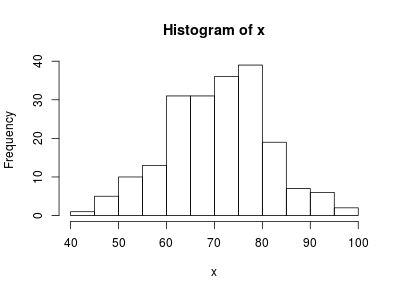
\includegraphics[scale=.8]{./diagrams/histogram.png}
\end{figure}
\end{frame}

\begin{frame}
  \frametitle{Characterizing Data Sets}
  The following serve to characterize data sets without listing the
  data:
  \begin{itemize}
  \item measures of centre
  \item measures of dispersion
  \item measures of position
  \end{itemize}
\end{frame}

\begin{frame}
  \frametitle{Measures of Centre: Mean}
  \begin{equation}
    \label{eq:daechuev}
    \mbox{mean}=\frac{\sum{}x}{n}
  \end{equation}
  where $n$ is the number of data points in your quantitative data set
  and $x$ is your data set. Mathematically speaking, $x$ is an
  $n$-dimensional vector $x=(x_{1},{\ldots},x_{n})$ and $\sum{}x$
  means
  \begin{equation}
    \label{eq:aethecux}
    \sum{}x=x_{1}+{\ldots}x_{n}
  \end{equation}
Often, we write $\mu$ for the mean of a
  population and $\bar{x}$ for the mean of a sample.
\end{frame}

\begin{frame}
  \frametitle{Frequency Distributions}
Often, data is provided in the form of a frequency distribution. For
example, when I asked a class of statistics students about the number
of countries they had visited in their lifetime, the response was as
follows (given as an R command),
\begin{alltt}
\small
cn<-c(5,4,7,3,6,4,3,4,2,4,4,2,4,3,2,4,4)
\end{alltt}
A more intelligible way to display the data is to provide a frequency
distribution.
\begin{alltt}
> table(cn)\newline
cn\newline
2 3 4 5 6 7 \newline
3 3 8 1 1 1
\end{alltt}
There are 3 people who have been to 2 countries, 3 people who have
been to 3 countries, 8 people who have been to 4 countries, 1 person
who has been to 5 countries, and so on.
\end{frame}

\begin{frame}
  \frametitle{Calculating the Mean from a Frequency Distribution}
If you have a frequency distribution (usually of a sample, so we will
call the mean $\bar{x}$), the mean is 
\begin{equation}
  \label{eq:eogheivi}
  \bar{x}=\frac{\sum{}\left(f\cdot{}x\right)}{\sum{}f}
\end{equation}
For the example in the last slide,
\begin{equation}
  \label{eq:uevuemoo}
  \bar{x}=\frac{2\cdot{}3+3\cdot{}3+4\cdot{}8+5\cdot{}1+6\cdot{}1+7\cdot{}1}{3+3+8+1+1+1}\approx{}3.82
\end{equation}
In R, you can also simply use the command \texttt{mean}. Notice that
\texttt{mean(x)} and \texttt{sum(x)/length(x)} will give you the same
number.
\end{frame}

\begin{frame}
  \frametitle{Exercises}
  {\ubung} Find the mean of the following five counts for Chips Ahoy
  chocolate chip cookies: 22 chips, 22, chips, 26 chips, 24 chips, and
  23 chips.

  \bigskip

  {\ubung} Anne measures the temperature in her walk-in freezer. She
  measures $-23^{\circ}$C once; $-22^{\circ}$C 31 times;
  $-21^{\circ}$C 13 times; $-20^{\circ}$C 7 times; $-18^{\circ}$C
  twice. What is the mean temperature given this dataset?
\end{frame}

\begin{frame}
  \frametitle{Measures of Centre: Median}
The median is the value in the middle. If there is an even number of
data points, the median is the mean of the two data points in the
middle. To find the median, sort the data points. For example, the
numbers of countries visited are

\medskip

\begin{tabular}{|c|c|c|c|c|c|c|c|c|c|c|c|c|c|c|c|c|}\hline
2&2&2&3&3&3&4&4&\alert{4}&4&4&4&4&4&5&6&7 \\ \hline
\end{tabular}

\medskip

The value in the middle is the number 4, which is also the median of
the data. It is quite similar to the mean, which is approximately 3.82.
\end{frame}

\begin{frame}
  \frametitle{Difference Between Mean and Median}
Imagine we had one more student in the class who was a world traveler.
She had visited 112 countries! The mean is now
\begin{equation}
  \label{eq:zephahwu}
  \bar{x}=\frac{\sum{}x}{n}=\frac{177}{18}\approx{}9.83
\end{equation}
A mean of 9.83 is no longer a good summary of the data. Let's see if
the median does better.

\medskip

\begin{tabular}{|c|c|c|c|c|c|c|c|c|c|c|c|}\hline
2&2&{\ldots}&4&4&\alert{4}&\alert{4}&4&{\ldots}&6&7&112 \\ \hline
\end{tabular}

\medskip

The new median is $(4+4)/2=4$, which is a much better summary of the
data, pretty much ignoring the outlier.
\end{frame}

\begin{frame}
  \frametitle{Measures of Centre: Mode}
The \alert{mode} of a data set is the value that occurs with the
greatest frequency. In the numbers of countries visited example the
mode is clearly 4. To be precise, the mode of a data set is itself a
set of numbers. A data set can have one mode, as in our example, but
if more values are repeated the same number and a maximum number of
times, they are all modes. If no data point is repeated, the data set
has no mode.
\end{frame}

\begin{frame}
  \frametitle{Measures of Centre: Midrange}
The \alert{midrange} is the midpoint between the maximum and the
minimum data points. It is very sensitive to outliers! For example,
\begin{equation}
  \label{eq:nahjuise}
  \mbox{midrange}=\frac{7+2}{2}=4.5
\end{equation}
without the outlier, and
\begin{equation}
  \label{eq:foofieng}
  \mbox{midrange}=\frac{112+2}{2}=57
\end{equation}
with the outlier in the numbers of countries visited example.
\end{frame}

\begin{frame}
  \frametitle{Measures of Dispersion: Motivation}
Have a look at these two different data sets.
\begin{alltt}
x1<-c(12,12,12,12,12,12,11,12,12,13,12,12,12,12)
\end{alltt}
and
\begin{alltt}
x2<-c(15,10,14,7,17,15,11,18,12,12,15,9,7,6)
\end{alltt}
The mean of both data sets is 12. The median of both data sets is 12.
However, something about these two data sets is different. \texttt{x2}
is more dispersed than \texttt{x1}, which means that the data is
spread out more. There is more variation in \texttt{x2}. We try to
capture this variation by finding measures of dispersion.
\end{frame}

\begin{frame}
  \frametitle{Measures of Dispersion: Range}
One very simple measure of dispersion is the \alert{range}, which is
just the lowest value subtracted from the highest value. 
\begin{equation}
  \label{eq:ungoliex}
  \mbox{range of \texttt{x1} }=13-11=2
\end{equation}
\begin{equation}
  \label{eq:aengoore}
  \mbox{range of \texttt{x2} }=18-6=12
\end{equation}
The problem is outliers: they would change the range significantly
while many other data points would be ignored. Another possibility is
to count up the difference between data points and the mean. Can you
guess what the problem of this measure would be?
\end{frame}

\begin{frame}
  \frametitle{Measures of Dispersion: Midquartile}
The \alert{interquartile range} is a measure of dispersion which is not as
vulnerable to outliers as the range. The interquartile range is
visually best represented in a box-and-whiskers display. For the 200
students, the box-and-whiskers display is generated by the following R
Studio command,
\begin{alltt}
boxplot(x,range=0)
\end{alltt}
\texttt{range=0} means that the plot will not pay attention to
outliers. The default is \texttt{range=1.5}, which will show some
outliers. We will find out how to calculate quartiles in a moment when
we will talk about measures of position. The interquartile range is
the third quartile minus the first quartile, $Q3-Q1$. However, some
programs (such as R Statistics) use ways to calculate quartiles that
are not the same as ours (type 7 versus type 1). 
\end{frame}

% \begin{frame}
%   \frametitle{Box-and-Whiskers Display Without Outliers}
% \begin{figure}[h]
% \includegraphics[scale=.6]{./diagrams/box.png}
% \end{figure}
% \end{frame}

\begin{frame}
  \frametitle{Box-and-Whiskers Display with Outliers}
\begin{figure}[h]
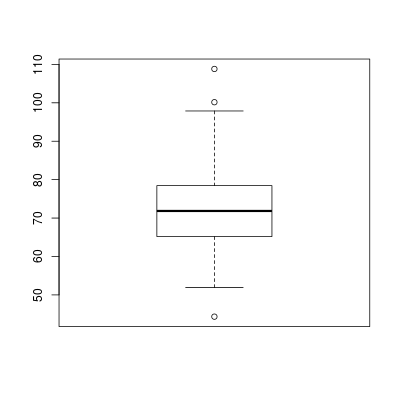
\includegraphics[scale=.6]{./diagrams/box1.png}
\end{figure}
\end{frame}

\begin{frame}
  \frametitle{Measures of Dispersion: Absolute Value of Deviation}
The difference between data points and the mean always sums to zero!
That is not helpful. If we want to make this measure of dispersion
more useful, we need to sum the \alert{absolute value of deviation}
\begin{equation}
  \label{eq:riquithu}
  \mbox{mean absolute deviation }=\frac{\sum{}\vert{}x-\bar{x}\vert}{n}
\end{equation}
For our examples \texttt{x1} and \texttt{x2}, the mean absolute
deviations are 2 and 44, respectively. Although at first glance this
measure of dispersion looks useful, it makes for very complicated
calculations that can be simplified by choosing a different way to
make all the distances between data points and mean positive: not the
absolute value, but the square of the distance.
\end{frame}

\begin{frame}
  \frametitle{Measures of Dispersion: Variance}
The \alert{variance} is calculated as follows,
\begin{equation}
  \label{eq:roongeef}
   \mbox{variance of a population }=\sigma^{2}=\frac{\sum{}(x-\mu)^{2}}{n}
\end{equation}
Something odd happens when we take the variance of a sample. If we
were to use equation (\ref{eq:roongeef}) to calculate the sample
variance for all possible samples of a population, the mean of these
sample variance would not equal the population variance. This means
that in this case the sample variance would be a \alert{biased
  estimator} of the population variance. We don't want that! To
correct for this problem and define a sample variance which is an
\alert{unbiased estimator} of the population variance, we introduce
\alert{Bessel's correction} and define
\begin{equation}
  \label{eq:ilosoama}
   \mbox{variance of a sample }=s^{2}=\frac{\sum{}(x-\bar{x})^{2}}{n-1}
\end{equation}
\end{frame}

\begin{frame}
  \frametitle{Measures of Dispersion: Standard Deviation}
One disadvantage of the variance is that it is not an intuitive
measurement of dispersion. If we take the square root of the variance,
then we get something similar to the absolute value of deviation,
which tells us approximately how far on average the data points are
from the mean. We call this measurement the \alert{standard
  deviation}
\begin{equation}
  \label{eq:boolaesh}
   \mbox{standard deviation of a population }=\sigma=\sqrt{\frac{\sum{}(x-\mu)^{2}}{n}}
\end{equation}
\begin{equation}
  \label{eq:xeiroong}
   \mbox{standard deviation of a sample }=s=\sqrt{\frac{\sum{}(x-\bar{x})^{2}}{n-1}}
\end{equation}
Why we still sometimes prefer the variance will become
clear on the next slide. The standard deviation, whether with or
without Bessel's Correction, is a biased estimator!
\end{frame}

\begin{frame}
  \frametitle{Bessel's Correction}
\begin{figure}[h]
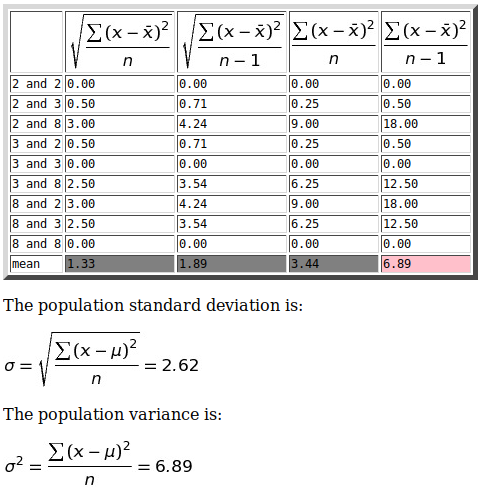
\includegraphics[scale=.45]{./diagrams/bessel.png}
\end{figure}
\end{frame}

\begin{frame}
  \frametitle{Calculating the Variance I}
It is easiest to calculate the variance using statistical software. In
R Studio, for example,
\begin{alltt}
> var(x1)\newline
[1] 0.1538462\newline
> var(x2)\newline
[1] 14.76923
\end{alltt}
and
\begin{alltt}
> sd(x1)\newline
[1] 0.3922323\newline
> sd(x2)\newline
[1] 3.843076
\end{alltt}
\end{frame}

\begin{frame}
  \frametitle{Calculating the Variance II}
When you do have to calculate the variance by hand, it is helpful to
use the following shortcut formula,
\begin{equation}
  \label{eq:eecheaxe}
s^{2}=\frac{\sum(x-\bar{x})^{2}}{n-1}=\frac{\sum{}x^{2}-\frac{\left(\sum{}x\right)^{2}}{n}}{n-1}
\end{equation}
because you do not have to keep entering the mean, which may contain
numerous significant digits.
\end{frame}

\begin{frame}
  \frametitle{Variance for a Frequency Distribution I}
Consider the data set \texttt{x3}
\begin{alltt}
4,4,2,2,4,3,3,3,1,4,4,1,2,2,2,4,2,1,2,1,1,2,3,3,2,3,3,3
\end{alltt}
We can summarize the data in a frequency distribution
\begin{alltt}
> table(x3)\newline
x3\newline
1 2 3 4 \newline
5 9 8 6 
\end{alltt}
\end{frame}

\begin{frame}
  \frametitle{Variance for a Frequency Distribution II}
Remember that in equation (\ref{eq:eogheivi}) we calculated the mean using a
formula for the frequency distribution,
\begin{equation}
  \label{eq:beingeip}
  \bar{x}=\frac{\sum{}\left(f\cdot{}x\right)}{\sum{}f}
\end{equation}
We can do the same for the variance and the standard deviation,
\begin{equation}
  \label{eq:iefoopoo}
  s^{2}=\frac{\sum{}\left(f\cdot{}x^{2}\right)-\frac{\left(\sum{}f\cdot{}x\right)^{2}}{\sum{}f}}{\sum{}f-1}
\end{equation}
Remember that $n=\sum{}f$.
\end{frame}

\begin{frame}
  \frametitle{Measures of Position: Quartiles}
Sometimes we want to know where a data point approximately ranks in
relation to other data points. For a more finely-grained measure of
position, we use percentiles. For a more coarsely-grained measure of
position, we use quartiles. Let's use again the R command
\begin{alltt}
  x<-round(rnorm(200,71,11)*100)/100
\end{alltt}
for the grades of 200 students in a course. On the next slide, you can
see the random numbers generated when I just now ran this command in R Studio.
\end{frame}

\begin{frame}
  \frametitle{Measures of Position: Quartiles}
\begin{alltt}
\footnotesize
  [1]  58.52  74.38  80.79  84.24  86.61  70.92  86.98  76.02  70.67  66.10\newline
 [11]  62.01  63.41  76.33  68.60  73.50  64.15  85.85  86.22  76.80  71.12\newline
 [21]  78.29  52.77  81.25  57.98  66.09  92.43  71.19  65.26  96.96  55.92\newline
 [31]  71.87  70.31  66.84  69.42  67.90  66.46  69.87  72.35  76.83  58.30\newline
 [41]  61.90  57.93  74.90  97.23  87.41  74.86  77.69  63.41  53.55  78.95\newline
 [51]  78.76  71.04  68.63  70.10  77.72  94.69  64.18  76.67  70.97  83.96\newline
 [61]  70.93  75.89  65.19  60.34  64.89  81.38  65.59  72.89  74.22  64.68\newline
 [71]  54.10  84.13  79.10  59.91  74.13  60.49  72.70  68.50  87.30  75.63\newline
 [81]  83.24  71.80  75.54  64.11  77.46  82.05  74.20  72.45  75.03  53.60\newline
 [91]  54.20  65.16  81.77  63.27  57.38  83.93  72.36  63.62  73.02  72.18\newline
[101]  54.66  84.89  58.05  70.27  80.31  76.43  70.66  71.31  86.39  77.85\newline
[111]  73.52  68.07  44.34  62.52  81.15  70.20  76.16  86.35  64.60  85.13\newline
[121]  61.21  65.25  72.94  61.48  90.48  80.50 108.81  57.91  73.53  65.53\newline
[131]  58.08  78.47  75.61  51.90  76.72  70.57  65.18  90.92  86.01  68.36\newline
[141]  78.16  54.97  81.10  75.30  52.39  68.64  82.96  71.82  80.44  59.15\newline
[151] 100.15  54.56  52.91  67.48  75.07  61.07  71.14  58.55  84.35  67.56\newline
[161]  94.91  78.32  70.50  75.73  67.25  71.49  62.55  68.54  59.55  63.01\newline
[171]  65.63  83.72  70.64  82.58  71.13  69.20  77.55  74.76  72.95  61.53\newline
[181]  73.04  84.79  64.35  85.49  78.86  56.27  74.11  97.87  72.58  92.96\newline
[191]  72.99  66.93  78.41  69.93  67.88  80.88  70.84  69.55  74.69  89.32
\end{alltt}
\end{frame}

\begin{frame}
  \frametitle{Measures of Position: Quartiles}
  Let's say you are student number 111, and your score is 73.52\%. The
  students are divided up into four groups of approximately the same
  size. The first quartile $Q_{1}$ is the score which divides the
  first group (with the lowest scores) from the second group. The
  second quartile $Q_{2}$ is the median and divides the second group
  from the third group. The third quartile $Q_{3}$ is the score which divides the
  third group from the fourth group (with the highest scores). 
\end{frame}

\begin{frame}
  \frametitle{Measures of Position: Quartiles}
  To calculate the quartiles you have to rank the data and find the
  corresponding scores, just as you did with the median. Or you use
  statistics software to check out the summary.
\begin{alltt}
> summary(x)\newline
   Min. 1st Qu.  Median    Mean 3rd Qu.    Max. \newline
  44.34   65.19   71.84   72.34   78.42  108.80 
\end{alltt}
\end{frame}

\begin{frame}
  \frametitle{Measures of Position: Quartiles}
  The second quartile is the median. The first quartile separates the
  bottom quarter of the data from the data group that scores higher
  than the bottom quarter and lower than the median. Let $n$ be the
  number of data points. Multiply $n$ by $1/4$ for the first quartile.
  If the result is a whole number $m$, then the first quartile is the
  mean of the two data points in the $m$-th and the $m+1$-th position
  from the bottom. If the result is not a whole number, round up to
  the whole number $m$ and the first quartile is the data point in the
  $m$-th position from the bottom.

  For the third quartile, multiply $n$ by $3/4$.
  If the result is a whole number $m$, then the third quartile is the
  mean of the two data points in the $m$-th and the $m+1$-th position
  from the bottom. If the result is not a whole number, round up to
  the whole number $m$ and the third quartile is the data point in the
  $m$-th position from the bottom.
\end{frame}

\begin{frame}
  \frametitle{Measures of Position: Percentiles}
Percentiles work just like quartiles, using the number 100 instead of
the number 4. Student number 111 turned out to be in the third
group because her score was better than the median but worse than the
third quartile. If we sort the data with the R Studio command
\begin{alltt}
sort(x)
\end{alltt}
we discover that student number 111 is in 115th position (counting
from the bottom), which is the 58th percentile. To find the $k$-th
percentile use
\begin{equation}
  \label{eq:phaecoab}
  \frac{n\cdot{}k}{100}
\end{equation}
For example, the 90th percentile $P_{90}$ is the mean between the 180th and the
181st data point ranked from the bottom (in our case, 85.93\%). As a
reference point, $P_{50}=Q_{2}=$median.
\end{frame}

\begin{frame}
  \frametitle{Percentiles Flow Chart I}
\begin{figure}[h]
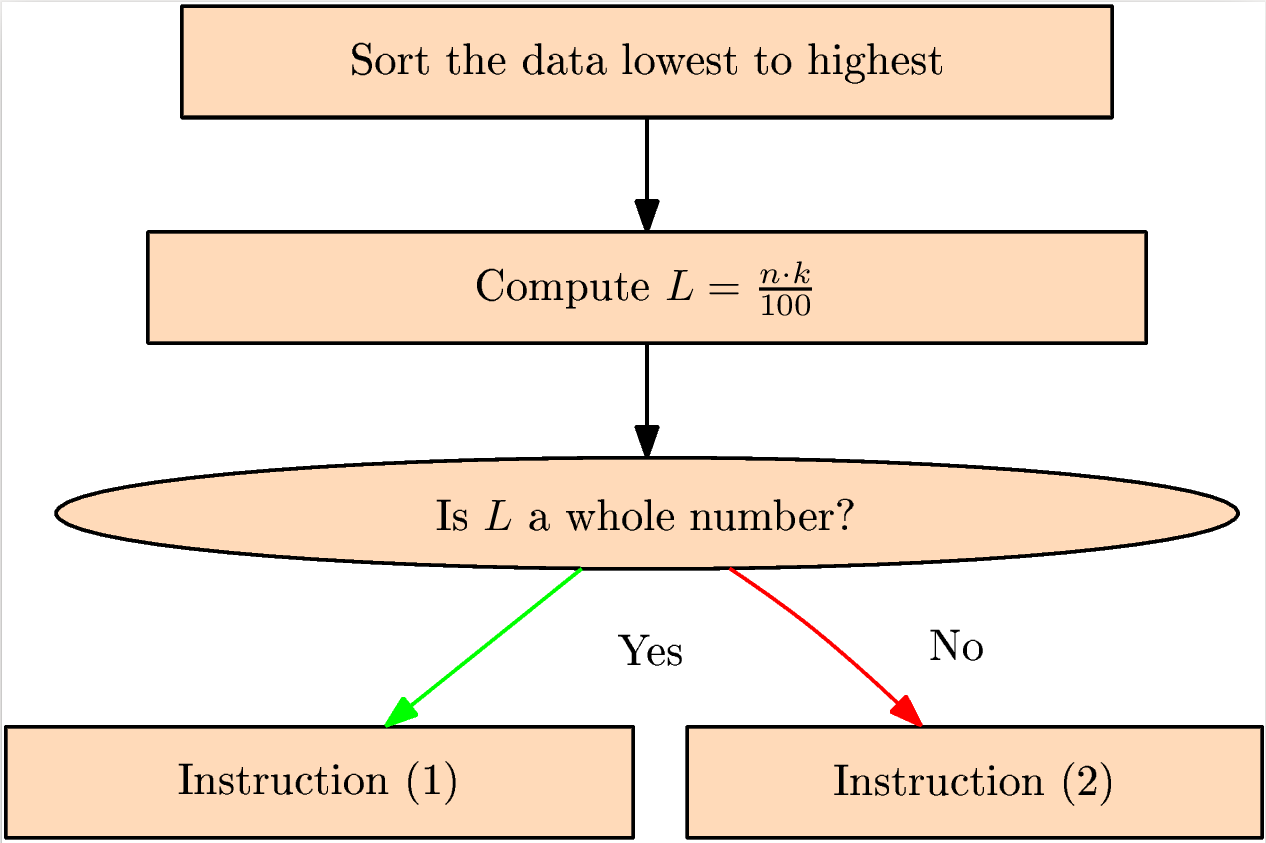
\includegraphics[scale=.15]{./diagrams/percentile.png}
\end{figure}
Instruction (1): The value of the $k$-th percentile $P_{k}$ is midway
between the $L$-th value and the next value in the sorted set of data.
Find $P_{k}$ by adding the $L$-th value and the next value and
dividing the total by $2$.
\end{frame}

\begin{frame}
  \frametitle{Percentiles Flow Chart II}
\begin{figure}[h]
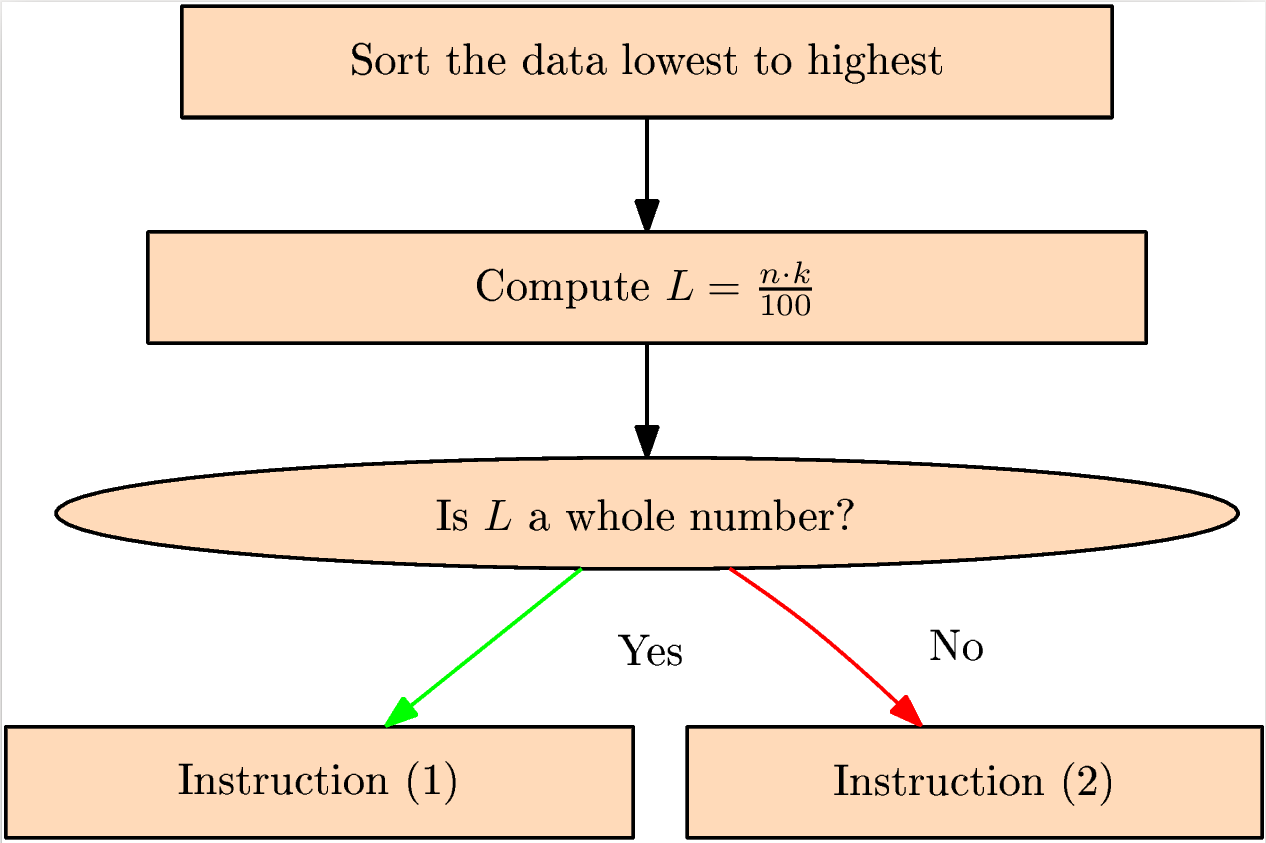
\includegraphics[scale=.15]{./diagrams/percentile.png}
\end{figure}
Instruction (2): Change $L$ by rounding it up to the next larger
whole number. The value of $P_{k}$ is the $L$-th value, counting
from the lowest.
\end{frame}

\begin{frame}
  \frametitle{Definitions}
  \begin{description}
  \item[event] An event is any collection of results or outcomes of a
    procedure.
  \item[sample space] The sample space for a procedure consists of all
    possible simple events. That is, the sample space consists of all
    outcomes that cannot be broken down any further. The symbol for
    the sample space is $\Omega$. 
  \item[complement] The complement of event $A$ is $\urcorner{}A$ and
    consists of all outcomes in which $A$ does not occur.
  \end{description}
\end{frame}

\begin{frame}
  \frametitle{Logic and Sets I}
  \begin{enumerate}
  \item<1-> $A\vee{}B$ is the event ``either $A$ or $B$ happens.''
  \item<2-> $A\wedge{}B$ is the event ``both $A$ and $B$ happens.''
  \item<3-> $\urcorner{}A$ is the event ``$A$ does not happens.''
  \item<4-> $\Omega$ and $\emptyset$ are events; they are called
    `tautology' and `contradiction,' respectively.
  \end{enumerate}
\end{frame}

\begin{frame}
  \frametitle{Logic and Sets II}
  The logical statement $A\vee{}B$ corresponds to the union of sets
  $A\cup{}B$ if $A$ and $B$ are understood as sets of simple events.

\medskip

  The logical statement $A\wedge{}B$ corresponds to the intersection of sets
  $A\cap{}B$ if $A$ and $B$ are understood as sets of simple events.

\medskip

Events $A$ and $B$ are \alert{disjoint} (or \alert{mutually
  exclusive}) if they cannot occur together. In set theory, we can
express this by saying that they are disjoint if and only if
$A\cap{}B=\emptyset$.

Think of dice rolls as an example. $\Omega=\{1,2,3,4,5,6\}$. Event $A$
may be $\{1,2,3\}$, and event $B$ may be $\{2,4,6\}$. What, then, are
events $A\cup{}B$ and $A\cap{}B$?
\end{frame}

\begin{frame}
  \frametitle{Definition of Probability}
Let $\Omega$ be a set of simple events. An event $A$ is then a subset
of $\Omega$. A function $P$ from the collection of all these subsets
(sometimes called the power set of $\Omega$) to the real numbers is a
\alert{probability function} if the following three conditions are
fulfilled.
\begin{enumerate}
\item<1-> $P(A)\geq{}0$ for all events $A$.
\item<2-> $P(\Omega)=1$.
\item<3->
  $P(A\cup{}B)=P(A)+P(B)$
  for any collection of disjoint events $A,B$.
\end{enumerate}
\end{frame}

\begin{frame}
  \frametitle{Basic Theorems of Probability}
Here are some basic theorems that follow from the conditions.
\begin{block}{Rule of Complementary Events}
  $P(\urcorner{}A)=1-P(A)$\mbox{ for all events }A
\end{block}
This immediately implies that $P(\emptyset)=0$ since
$\emptyset=\urcorner\Omega$.
\begin{block}{Addition Rule}
  $P(A\cup{}B)=P(A)+P(B)-P(A\cap{}B)$
\end{block}
\end{frame}

\begin{frame}
  \frametitle{Conditional Probability}
Conditional probability of $A$ conditional on $B$ is defined as follows,
\begin{equation}
  \label{eq:iekeengi}
  P(B|A)=\frac{P(A\cap{}B)}{P(A)}
\end{equation}
This theorem follows immediately,
\begin{block}{Multiplication Rule}
  $P(A\cap{}B)=P(A)\cdot{}P(B|A)$
\end{block}
Two events $A$ and $B$ are \alert{independent} if and only if
$P(A\cap{}B)=P(A)\cdot{}P(B)$. Given the multiplication rule, this is
equivalent to saying that $P(A|B)=P(A)$ and $P(B|A)P(B)$.
\end{frame}

\begin{frame}
  \frametitle{Rules}
  \begin{block}{Addition Rule}
    When $A$ and $B$ are \emph{disjoint}, then
    $P(A\cup{}B)=P(A)+P(B)$; otherwise use
    $P(A\cup{}B)=P(A)+P(B)-P(A\cap{}B)$
\end{block}
\bigskip
\begin{block}{Multiplication Rule}
  When $A$ and $B$ are \emph{independent}, then
  $P(A\cap{}B)=P(A)\cdot{}P(B)$; otherwise use
  $P(A\cap{}B)=P(A|B)\cdot{}P(B)$
\end{block}
\end{frame}

\begin{frame}
  \frametitle{Mendel's Law of Separation}
\begin{figure}[h]
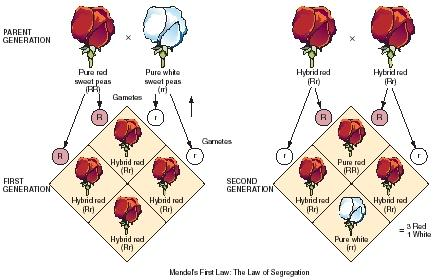
\includegraphics[scale=.75]{./diagrams/mendel.jpg}
\end{figure}
\end{frame}

\begin{frame}
  \frametitle{Exercises}
{\ubung} Your friend tosses two coins. You don't see the
coins, but your friend tells you that at least one of them landed
heads. What is the probability that they both landed heads?

{\ubung} Alice and Branden have brown eyes. Their son Joel has blue
eyes. What is the probability that their next child will have blue
eyes as well?

{\ubung} In a sample of 207 adults, 43 are smokers. What
is the probability of choosing a person at random who is a smoker?
\end{frame}

\begin{frame}
  \frametitle{Exercises}
{\ubung} A game show host asks you a multiple choice
question with four answers A, B, C, and D. If you make a random guess,
what is your probability of getting the correct answer?

{\ubung} In a country far away, all parents want to have
girls. The probability of having a girl is 50\%. All parents have boys
until they have a girl. What would you expect to be the proportion of
girls in that country?

{\ubung} The government found out that 102 out of 810
luggage scales at the airport are defective. If you choose 2 luggage
scales at random \emph{with replacement}, what is the probability that
they are both defective? If you choose 2 luggage scales at random
\emph{without replacement}, what is the probability that they are both
defective?
\end{frame}

\begin{frame}
  \frametitle{Tree Diagrams I}
{\ubung} The probability that BCIT hires a person on a
particular weekday is the same as any other weekday. What is the
probability that two randomly selected employees were both hired on a
Monday? What is the probability that two randomly selected employees
were both hired on the same weekday?

{\ubung} In a group of people, 492 would choose a window
seat on an airplane, 8 would choose a middle seat, and 306 would
choose an aisle seat. What is the probability of randomly choosing a
person who would not choose a middle seat? What is the probability of
randomly choosing two people who would not choose a middle seat? What
is the probability of randomly choosing twenty-five people who would
not choose a middle seat?
\end{frame}

\begin{frame}
  \frametitle{Tree Diagrams II}
{\ubung} What is the probability of rolling a sum of 9 on
two dice rolls?

{\ubung} What is the probability of having two girls and
three boys when there are five children and the probability of having
a boy is 50\%?
\end{frame}

\begin{frame}
  \frametitle{Tree Diagrams}
You can use independence and mutual exclusion to draw tree diagrams.
\begin{figure}[h]
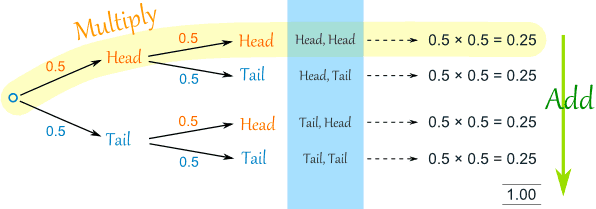
\includegraphics[scale=.5]{./diagrams/tree.png}
\end{figure}
\end{frame}

\begin{frame}
  \frametitle{Exercise Tree Diagram}
{\ubung} You have two coaches, Sam and Alex. When Sam
coaches the team, your proability of being the goalkeeper is 50\%. When Alex
coaches the team, your proability of being the goalkeeper is 30\%. The
probability that Sam (rather than Alex) will coach your team today is
60\%. What is the probability that you will be goalkeeper?
\end{frame}

\newcommand{\sam}{.65}

\begin{frame}
  \frametitle{Sam and Alex I}
\begin{figure}[h]
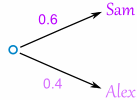
\includegraphics[scale=\sam]{./diagrams/sam1.png}
\end{figure}
\end{frame}

\begin{frame}
  \frametitle{Sam and Alex II}
\begin{figure}[h]
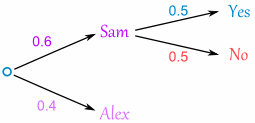
\includegraphics[scale=\sam]{./diagrams/sam2.png}
\end{figure}
\end{frame}

\begin{frame}
  \frametitle{Sam and Alex III}
\begin{figure}[h]
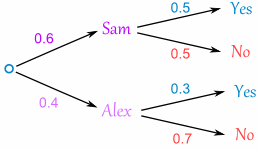
\includegraphics[scale=\sam]{./diagrams/sam3.png}
\end{figure}
\end{frame}

\begin{frame}
  \frametitle{Sam and Alex IV}
\begin{figure}[h]
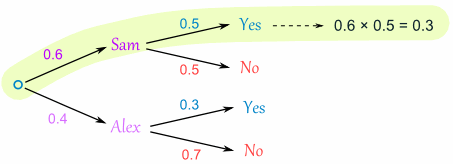
\includegraphics[scale=\sam]{./diagrams/sam4.png}
\end{figure}
\end{frame}

\begin{frame}
  \frametitle{Sam and Alex V}
\begin{figure}[h]
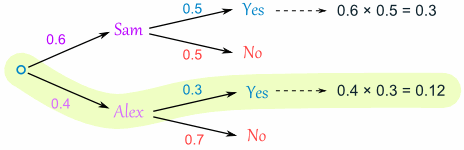
\includegraphics[scale=\sam]{./diagrams/sam5.png}
\end{figure}
\end{frame}

\begin{frame}
  \frametitle{Sam and Alex VI}
\begin{figure}[h]
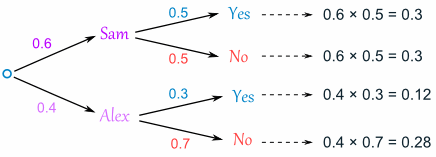
\includegraphics[scale=\sam]{./diagrams/sam6.png}
\end{figure}
\end{frame}

\begin{frame}
  \frametitle{How to Solve Probability Problems}
In summary, here are some strategies to solve probability problems.
\begin{enumerate}
\item<1-> Count simple events. If the simple events are all equally
  probable, then the probability of event $A$ is the number of simple
  events in $A$ divided by the total number of simple events, so
  $P(A)=\#A/\#\Omega$.
\item<2-> Make sure to watch for independence and mutual exclusion.
  Whenever events are independent or mutually exclusive (disjoint),
  you can use $P(A\cap{}B)=P(A)P(B)$ or $P(A\cup{}B)=P(A)+P(B)$,
  respectively.
\item<3-> If events are not mutually exclusive, you can use the
  addition rule $P(A\cup{}B)=P(A)+P(B)-P(A\cap{}B)$.
\item<4-> If events are not independent, you can use conditional
  probabilities in $P(A\cap{}B)=P(A)P(B|A)$.
\item<5-> If you are dealing with events that are independent and
  mutually exclusive, it is often useful to draw a tree diagram.
\end{enumerate}
\end{frame}

\begin{frame}
  \frametitle{How to Solve Probability Problems}
In summary, here are some strategies to solve probability problems.
\begin{enumerate}
\item Count simple events. If the simple events are all equally
  probable, then the probability of event $A$ is the number of simple
  events in $A$ divided by the total number of simple events, so
  $P(A)=\#A/\#\Omega$.
\item Make sure to watch for independence and mutual exclusion.
  Whenever events are independent or mutually exclusive (disjoint),
  you can use $P(A\cap{}B)=P(A)P(B)$ or $P(A\cup{}B)=P(A)+P(B)$,
  respectively.
\item If events are not mutually exclusive, you can use the
  addition rule $P(A\cup{}B)=P(A)+P(B)-P(A\cap{}B)$.
\item If events are not independent, you can use conditional
  probabilities in $P(A\cap{}B)=P(A)P(B|A)$.
\item If you are dealing with events that are independent and
  mutually exclusive, it is often useful to draw a tree diagram.
\end{enumerate}
\end{frame}

\begin{frame}
  \frametitle{Permutations and Combinations}
When we use
\begin{equation}
  \label{eq:adeiquah}
  P(A)=\frac{\#A}{\#\Omega}
\end{equation}
it can be difficult to do the counting. Formulas for permutations and
combinations help. For \alert{permutations}, order matters. The
permutations of the letters ABC are ABC, ACB, BAC, BCA, CAB, and CBA.
For \alert{combinations}, order does not matter. There are four
combinations of three letters for the four letters ABCD: ABC, ABD,
ACD, and BCD.
\end{frame}

\begin{frame}
  \frametitle{Rule I: Fundamental Counting Rule}
  The fundamental counting rule says that if there are $m$ ways for
  the first event to occur and $n$ ways for the second event to occur,
  then there are $m\cdot{}n$ combinations of these two events to
  occur.

\bigskip

\textbf{Example:} How many postal codes are possible in Canada?
\end{frame}

\begin{frame}
  \frametitle{Rule II: Factorial Rule}
Factorials are defined as follows,
\begin{equation}
  \label{eq:iepeejae}
  0!=1\mbox{ and }(n+1)!=(n+1)\cdot{}n!\mbox{ for all natural numbers }n
\end{equation}
For example, $6!=1\cdot{}2\cdot{}3\cdot{}4\cdot{}5\cdot{}6=720$.

\bigskip

The factorial rule says that there are $n!$ ways to arrange $n$
different items.

\bigskip

\textbf{Example:} You have to rank six Canadian prime ministers in
chronological order. If you know nothing about history, what is your
probability of ranking them correctly?
\end{frame}

\begin{frame}
  \frametitle{Rule III: Permutations Rule}
When you select $r$ items from $n$ available items \alert{without
  replacement}, then there are
\begin{equation}
  \label{eq:eahaikee}
  \frac{n!}{(n-r)!}
\end{equation}
permutations.

\bigskip

\textbf{Example:} How many ten-letter words are there without
repeating letters?
\end{frame}

\begin{frame}
  \frametitle{Rule IV: Combinations Rule}
When you select $r$ items from $n$ available items \alert{without
  replacement}, then there are
\begin{equation}
  \label{eq:aibireik}
  \frac{n!}{(n-r)!r!}
\end{equation}
combinations.

\bigskip

\textbf{Example:} How many different samples of $n=10$ are there in a
population of 30?
\end{frame}

\begin{frame}
  \frametitle{Counting Exercises I}
(1) Starting with 26 Latin letters, how many five-letter words
(meaningful or not) are there (with repetitions)? How many are there
without repetition?
\end{frame}

\begin{frame}
  \frametitle{Counting Exercises II}
(2) How many four digit numbers are there with no repeating digits?
\end{frame}

\begin{frame}
  \frametitle{Counting Exercises III}
(3) If you were to read the seven Harry Potter books in random order,
what is the probability that you read them in the correct order?
\end{frame}

\begin{frame}
  \frametitle{Counting Exercises IV}
(4) The Rankin Family wants to make a Best Of CD out of their 27
songs. The CD is to have 12 songs on it. How many possibilities of
choosing 12 out of 27 songs are there (order does not matter)?
\end{frame}

\begin{frame}
  \frametitle{Counting Exercises V}
(5) Justin Trudeau wants to visit 4 out of the 10 Canadian provinces.
His advisor rattles off all the possible routes (order matters), one
per ten seconds. How long did it take her to do so?
\end{frame}

\begin{frame}
  \frametitle{Counting Exercises VI}
(6) Lotto 649 draws 6 out of 49 numbers (order does not matter). What
is your chance of winning? What is your chance of getting 5 numbers
correctly?
\end{frame}

\begin{frame}
  \frametitle{xkcd on Bayes' Formula}
\begin{figure}[h]
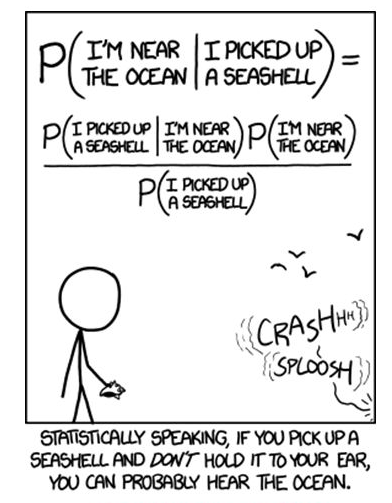
\includegraphics[scale=.5]{./diagrams/xkcd_bayes1.png}
\end{figure}
\end{frame}

\begin{frame}
  \frametitle{Two Examples}
Here are two of my own examples.
http://psycnet.apa.org/record/1975-11611-001 and
https://derstandard.at/2000076668166/Mythos-oder-wahr-Durch-Abschrecken-lassen-sich-Eier-besser-schaelen

For the second one: What is the probability that an egg is fresh when
it is a crater egg? For the first one: What is the probability of
being attractive when you are accepted?
\end{frame}

\begin{frame}
  \frametitle{Conditional Probability}
Let's remember what conditional probability means.
% \begin{equation}
%   \label{eq:ohyeweeb}
%   P(B|A)=\frac{P(B\cap{}A}{P(A)}
% \end{equation}
\begin{figure}[h]
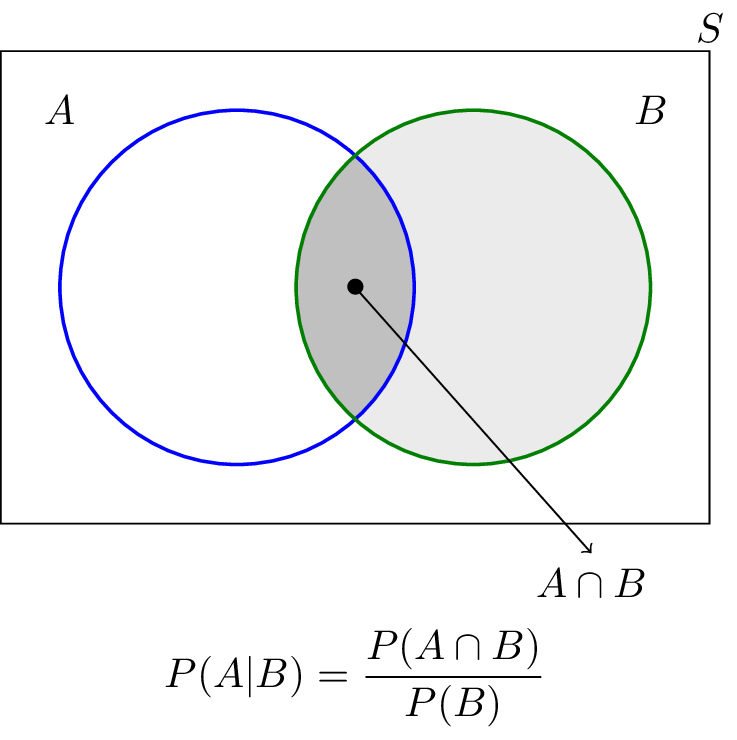
\includegraphics[scale=.25]{./diagrams/conditional_b.png}
\end{figure}
\end{frame}

\begin{frame}
  \frametitle{Multiplication Rule}
  Remember the thief who wants to crack the four-digit PIN of a bank
  card. Let $A$ be the event that she successfully cracks the PIN. If
  $A_{1}$ is the event that she succeeds on her first attempt (and so
  on for $A_{2}$ and $A_{3}$), then
\begin{equation}
  \label{eq:ragheidu}
  P(A)=P(A_{1}\cup{}A_{2}\cup{}A_{3})=P(A_{1})+P(A_{2})+P(A_{3})=0.003
\end{equation}
because $A_{1},A_{2},A_{3}$ are disjoint. We are assuming that her
attempts happen \alert{without replacement}. Therefore,
$A_{1},A_{2},A_{3}$ are not independent, and the correct application of
the multiplication rule is
\begin{equation}
  \label{eq:mohghunu}
  P(A)=1-P(\urcorner{}A)=\notag
\end{equation}
\begin{equation}
  \label{eq:yoobaegh}
  1-P(\urcorner{}A_{1})\cdot{}P(\urcorner{}A_{2}|\urcorner{}A_{1})\cdot{}P(\urcorner{}A_{3}|\urcorner{}A_{1}\cap{}\urcorner{}A_{2})=0.003
\end{equation}
\end{frame}

\begin{frame}
  \frametitle{Law of Total Probability}
It is often easier to calculate conditional probabilities than
unconditional probabilities. To express one by the other use the
\alert{law of total probability},
\begin{equation}
  \label{eq:aefengah}
  P(A)=P(A|B)P(B)+P(A|\urcorner{}B)P(\urcorner{}B)
\end{equation}
This formula also applies when you split up $B$ into three or more
disjoint subsets that exhaust $B$. It follows from set theory.

\bigskip

\textbf{Example: }Suppose that two factories supply light bulbs to the
market. Factory X's bulbs work for over 5000 hours in 99\% of cases,
whereas factory Y's bulbs work for over 5000 hours in 95\% of cases.
It is known that factory X supplies 60\% of the total bulbs available.
What is the chance that a purchased bulb will work for longer than
5000 hours?
% Now we should be able to answer the question from last week: How many
% four digit numbers are there with no repeating digits?
\end{frame}

\begin{frame}
  \frametitle{Law of Total Probability}
\textbf{Example: }Suppose that two factories supply light bulbs to the
market. Factory X's bulbs work for over 5000 hours in 99\% of cases,
whereas factory Y's bulbs work for over 5000 hours in 95\% of cases.
It is known that factory X supplies 60\% of the total bulbs available.
What is the chance that a purchased bulb will work for longer than
5000 hours?

\bigskip

Let $X$ be the event that the light bulb is from factory X. Let $F$ be
the event that the bulb will work for longer than
5000 hours. Then
\begin{equation}
  \label{eq:uwahiamo}
  P(F)=P(F|X)P(X)+P(F|\urcorner{}X)P(\urcorner{}X)=\notag
\end{equation}
\begin{equation}
  \label{eq:siecafoo}
  0.99\cdot{}0.60+0.95\cdot{}0.40=0.974
\end{equation}
\end{frame}

\begin{frame}
  \frametitle{Law of Total Probability Exercises I}
What is the probability that the second card in a conventional
deck of cards is an ace?
\end{frame}

\begin{frame}
  \frametitle{Law of Total Probability Exercises II}
Suppose we have two hats: one has 4 red balls and 7 green balls,
the other has 11 red and 5 green. We toss an unfair coin (60/40 for
heads), if heads, pick a random ball from the first hat, if tails from
the second. What is the probability of getting a red ball?
\end{frame}

\begin{frame}
  \frametitle{Law of Total Probability Exercises III}
You have three bags that each contain 100 marbles:
\begin{itemize}
\item Bag 1 has 75 red and 25 blue marbles
\item Bag 2 has 60 red and 40 blue marbles
\item Bag 3 has 45 red and 55 blue marbles
\end{itemize}
I choose one of the bags at random and then pick a marble from the
chosen bag, also at random. What is the probability that the chosen
marble is red?
\end{frame}

\begin{frame}
  \frametitle{Some Interesting Cases}
  A group of police officers have breathalyzers displaying false
  drunkenness in 5\% of the cases in which the driver is sober.
  However, the breathalyzers never fail to detect a truly drunk
  person. One in a thousand drivers is driving drunk. Suppose the
  police officers then stop a driver at random, and force the driver
  to take a breathalyzer test. It indicates that the driver is drunk.
  We assume you don't know anything else about him or her. How high is
  the probability he or she really is drunk?
\end{frame}

\begin{frame}
  \frametitle{Some Interesting Cases}
  A room is full of engineers and lawyers (most of them are lawyers,
  90\%). The probability that an engineer enjoyed physics in school is
  80\%. The probability that a lawyer enjoyed physics in school is
  30\%. You ask someone in the room whether they enjoyed physics, and
  the answer is yes. Should you bet that this person is a lawyer, or
  should you bet that she is an engineer?
\end{frame}

\begin{frame}
  \frametitle{Some Interesting Cases}
You have a million food items, of which 1 in 1000 is contaminated. You
have a contamination test with a 2\% false positive rate and a 0.5\%
false negative rate. A food item tests positive for contamination.
What is the probability that it is contaminated?
\end{frame}

\begin{frame}
  \frametitle{Some Interesting Cases}
  In a city of 1 million inhabitants let there be 100 terrorists and
  999,900 non-terrorists. To simplify the example, it is assumed that
  all people present in the city are inhabitants. Thus, the base rate
  probability of a randomly selected inhabitant of the city being a
  terrorist is 0.0001, and the base rate probability of that same
  inhabitant being a non-terrorist is 0.9999. In an attempt to catch
  the terrorists, the city installs an alarm system with a
  surveillance camera and automatic facial recognition software.

The software has two failure rates of 1\%:
\begin{itemize}
\item The false negative rate: If the camera scans a terrorist, a bell
  will ring 99\% of the time, and it will fail to ring 1\% of the
  time.
\item The false positive rate: If the camera scans a non-terrorist, a
  bell will not ring 99\% of the time, but it will ring 1\% of the
  time.
\end{itemize}

Suppose now that an inhabitant triggers the alarm. What is the chance
that the person is a terrorist?
\end{frame}

\begin{frame}
  \frametitle{Bayes' Formula}
Consider the definition of conditional probability,
\begin{equation}
  \label{eq:ohyeweeb}
  P(B|A)=\frac{P(B\cap{}A)}{P(A)}
\end{equation}
Now notice that $P(B\cap{}A)=P(A\cap{}B)=P(B)P(A|B)$. That means that
\begin{equation}
  \label{eq:maifiepu}
  P(B|A)=\frac{P(B)P(A|B)}{P(A)}
\end{equation}
By the law of total probability we can replace the denominator to give
us \alert{Bayes' Formula}
\begin{equation}
  \label{eq:ohrughai}
  P(B|A)=\frac{P(B)P(A|B)}{P(A|B)P(B)+P(A|\urcorner{}B)P(\urcorner{}B)}
\end{equation}
\end{frame}

\begin{frame}
  \frametitle{Base Rate Fallacy Diagram}
\begin{figure}[h]
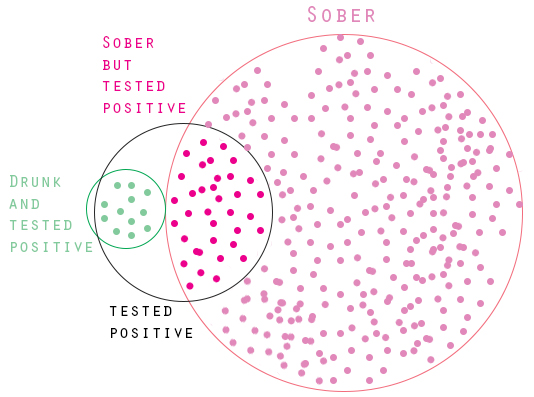
\includegraphics[scale=.4]{./diagrams/Detect-drunk-driving.jpg}
\end{figure}
\end{frame}

\begin{frame}
  \frametitle{Base Rate Fallacy Example}
  Let 100 out of 100,000 people have a disease. The test for this
  disease has a 5\% \alert{false positive} rate and a 5\% \alert{false
    negative} rate. If you test positive for this disease, what is
  your probability of actually having the disease. Consider the
  following \alert{contingency table} and then apply Bayes'
  formula.
\begin{figure}[h]
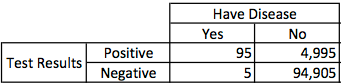
\includegraphics[scale=.7]{./diagrams/baserate3.png}
\end{figure}
\end{frame}

\begin{frame}
  \frametitle{Contingency Tables}
\begin{figure}[h]
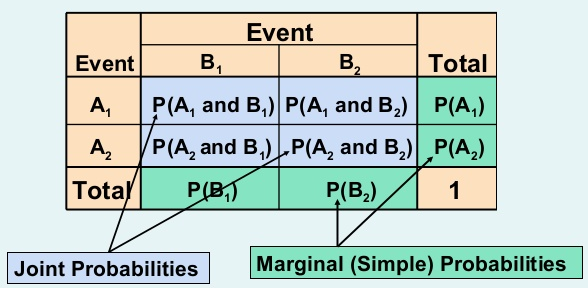
\includegraphics[scale=.5]{./diagrams/contingency1.png}
\end{figure}
\end{frame}

\begin{frame}
  \frametitle{Prison and Plea}
Here is a contingency table:
\begin{tabular}{|l|c|c|}\hline
  & Guilty Plea & Plea of Not Guilty \\ \hline
  Sentenced to Prison & 392 & 58 \\ \hline
  Not Sentenced to Prison & 564 & 14 \\ \hline
\end{tabular}
\end{frame}

\begin{frame}
  \frametitle{Prison and Plea}
Answer the following questions:
\begin{enumerate}
\item Find the probability of a randomly selected subject being
  sentenced to prison.
\item Find the probability of being sentenced to prison, given
  that the subject entered a plea of guilty.
\item Find the probability of being sentenced to prison, given
  that the subject entered a plea of not guilty.
\item Find the probability of a randomly selected subject being
  sentenced to prison or entering a plea of guilty.
\end{enumerate}
\end{frame}

\begin{frame}
  \frametitle{Prison and Plea}
Answer the following questions:
\begin{enumerate}
\setcounter{enumi}{4}
\item If two subjects are randomly selected, find the probability
  that they were both sentenced to prison.
\item If two subjects are randomly selected, find the probability
  that they both entered pleas of not guilty.
\item Find the probability of a randomly selected subject being
  entering a plea of not guilty or not being sentenced to prison.
\item Find the probability of a randomly selected subject being
  sentenced to prison and entering a plea of guilty.
\item Find the probability of a randomly selected subject not being
  sentenced to prison and not entering a plea of guilty.
\end{enumerate}
\end{frame}

\begin{frame}
  \frametitle{Exercises I}
% J.V. Uspensky, Introduction to Mathematical Probability, p40
Three urns contain respectively 1 white and 2 black balls; 3 white and
1 black ball; 2 white and 3 black balls. One ball is taken from each
urn. What is the probability that among the balls drawn there are 2
white and 1 black?
\end{frame}

\begin{frame}
  \frametitle{Exercises I}
% J.V. Uspensky, Introduction to Mathematical Probability, p40
Three urns contain respectively 1 white and 2 black balls; 3 white and
1 black ball; 2 white and 3 black balls. One ball is taken from each
urn. What is the probability that among the balls drawn there are 2
white and 1 black? Answer: $23/60$
\end{frame}

\begin{frame}
  \frametitle{Exercises II}
% Devore and Peck, Statistics, p247
A student has a box containing 25 computer disks, of which 15 are
blank and 10 are not. She randomly selects disks one by one and
examines each one, terminating the process only when she finds a blank
disk. What is the probability that she must examine at least two disks?
\end{frame}

\begin{frame}
  \frametitle{Exercises II}
% Devore and Peck, Statistics, p247
A student has a box containing 25 computer disks, of which 15 are
blank and 10 are not. She randomly selects disks one by one and
examines each one, terminating the process only when she finds a blank
disk. What is the probability that she must examine at least two
disks? Answer: 40\%
\end{frame}

\begin{frame}
  \frametitle{Exercises III}
% Devore and Peck, Statistics, p247
There are five faculty members in a certain academic department. These
individuals have 3, 6, 7, 10, and 14 years of teaching experience,
respectively. Two of these individuals are randomly selected to serve
on a committee. What is the probability that they have at least 15
years of teaching experience?
\end{frame}

\begin{frame}
  \frametitle{Exercises III}
% Devore and Peck, Statistics, p247
There are five faculty members in a certain academic department. These
individuals have 3, 6, 7, 10, and 14 years of teaching experience,
respectively. Two of these individuals are randomly selected to serve
on a committee. What is the probability that they have at least 15
years of teaching experience? Answer: 60\%
\end{frame}

\begin{frame}
  \frametitle{Exercises IV}
% Devore and Peck, Statistics, p249
Suppose three cards are selected from a well-mixed deck without
replacement. 
\begin{enumerate}
\item<1-> What is the probability that all three are hearts?
\item<2-> What is the probability that all three are from the same
  suit?
\item<3-> If five cards are dealt from a randomized deck, determine
  the probability that they are all hearts.
\end{enumerate}
\end{frame}

\begin{frame}
  \frametitle{Exercises IV}
% Devore and Peck, Statistics, p249
Suppose three cards are selected from a well-mixed deck without
replacement. 
\begin{enumerate}
\item What is the probability that all three are hearts? Answer: $1.29$\%
\item What is the probability that all three are from the same
  suit? Answer: $5.18$\%
\item If five cards are dealt from a randomized deck, determine
  the probability that they are all hearts. Answer: $0.0495$\%
\end{enumerate}
\end{frame}

\begin{frame}
  \frametitle{Exercises V}
% Devore and Peck, Statistics, p250
  A tennis coach has brought out 12 tubes of Penn balls and 8 tubes of
  Wilson balls for his class. If 5 tubes are randomly selected, what
  is the probability that all 5 are of the same brand?
\end{frame}

\begin{frame}
  \frametitle{Exercises V}
% Devore and Peck, Statistics, p250
  A tennis coach has brought out 12 tubes of Penn balls and 8 tubes of
  Wilson balls for his class. If 5 tubes are randomly selected, what
  is the probability that all 5 are of the same brand? Answer: $5.47$\%
\end{frame}

\begin{frame}
  \frametitle{Exercises VI}
\begin{figure}[h]
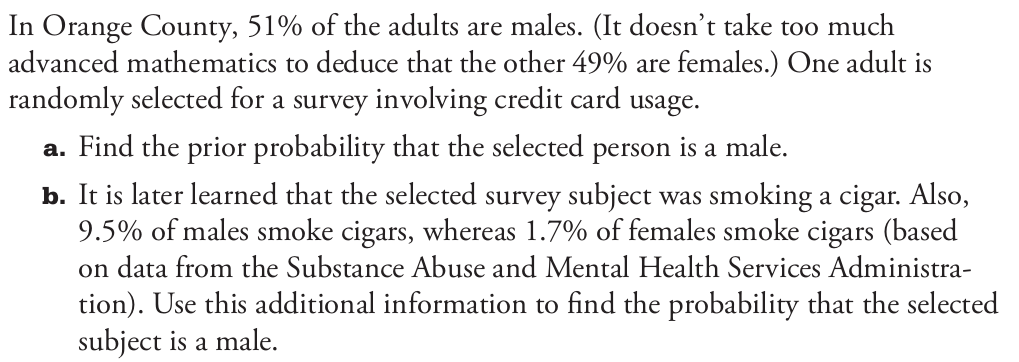
\includegraphics[scale=.32]{./diagrams/triola_bayes1.png}
\end{figure}
\end{frame}

\begin{frame}
  \frametitle{Exercises VI}
\begin{figure}[h]
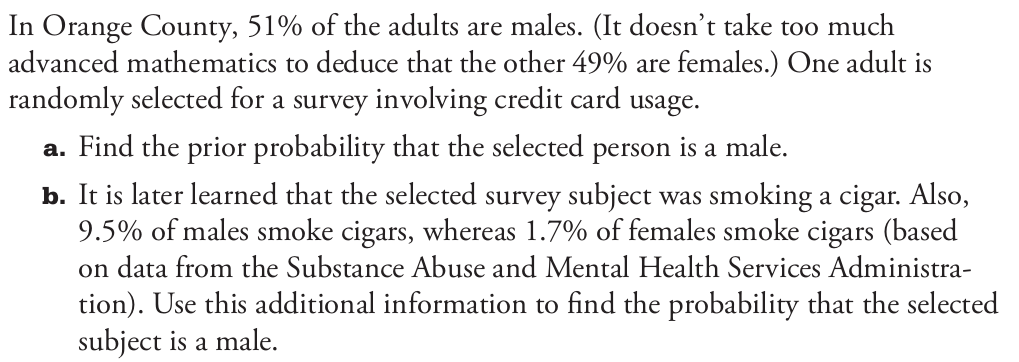
\includegraphics[scale=.32]{./diagrams/triola_bayes1.png}
\end{figure}
Answer: (a.) $51$\% (b.) $85.3$\%
\end{frame}

\begin{frame}
  \frametitle{Exercises VII}
\begin{figure}[h]
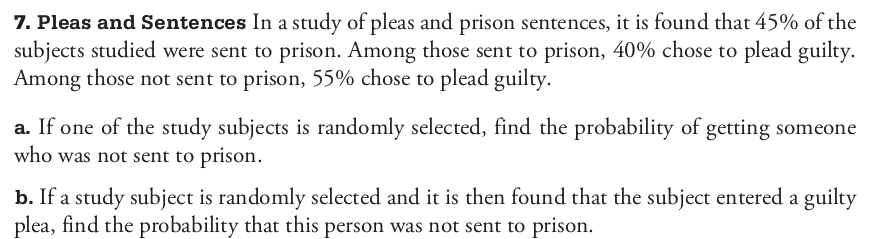
\includegraphics[scale=.36]{./diagrams/triola_bayes2.png}
\end{figure}
\end{frame}

\begin{frame}
  \frametitle{Exercises VII}
\begin{figure}[h]
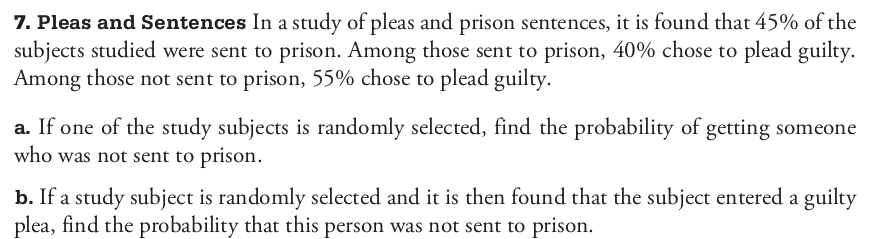
\includegraphics[scale=.36]{./diagrams/triola_bayes2.png}
\end{figure}
Answer: (a.) $55$\% (b.) $62.7$\%
\end{frame}

\begin{frame}
  \frametitle{Exercises VIII}
\begin{figure}[h]
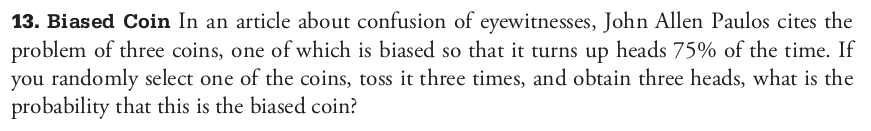
\includegraphics[scale=.36]{./diagrams/triola_bayes3.png}
\end{figure}
\end{frame}

\begin{frame}
  \frametitle{Exercises VIII}
\begin{figure}[h]
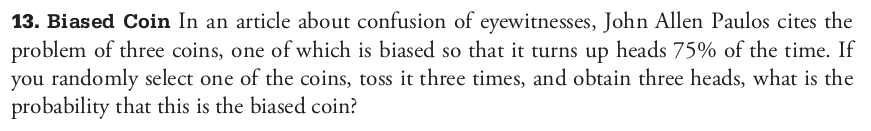
\includegraphics[scale=.36]{./diagrams/triola_bayes3.png}
\end{figure}
Answer: $62.8$\%
\end{frame}

\begin{frame}
  \frametitle{Probability Distributions: Concepts}
Here are some definitions.
\begin{description}
\item[random variable] A random variable is a variable (typically
  represented by $X$) that has a single numerical value, determined by
  chance, for each outcome of a procedure.
\item[probability distribution] A probability distribution is a
  description that gives the probability for each value of the random
  variable. It is often expressed in the format of a table, formula,
  or graph.
\end{description}
\end{frame}

\begin{frame}
  \frametitle{Probability Distributions: Discrete and Continuous}
\begin{description}
\item[discrete random variable] A \alert{discrete} random variable has
  a collection of values that is finite or countable.
\item[continuous random variable] A \alert{continuous} random variable has
  infinitely many values, and the collection of values is not
  countable.
\item[countability] This is best explained by example: the integers
  are countable, but the real numbers are not.
\end{description}
\end{frame}

\begin{frame}
  \frametitle{Discrete Probability Distributions}
  If there are a finite number of outcomes $X=a_{k}$ for
  $k=1,\ldots,n$, we can list the values of $P(X=a_{k})$ in a table. 

\bigskip

\beispiel{Coin Toss}\label{ex:ootiteij} let $X=1$ for heads and $X=0$
for tails. Then 

\bigskip

\begin{tabular}{|l|l|}\hline
  Event & Probability \\ \hline
  $X=1$ or $H$ & 0.50 \\ \hline
  $X=0$ or $T$ & 0.50 \\ \hline
\end{tabular}

\bigskip

When all the probabilities are equal, we call the probability
distribution a \alert{uniform distribution}.
\end{frame}

\begin{frame}
  \frametitle{Non-Uniform Discrete Probability Distributions}
  Some distribution probability distributions are not uniform.

\bigskip

  \beispiel{Number of Male Children}\label{ex:shaisail} Consider the
  two-child family. If $X$ is the random variable corresponding to the
  number of boys in the family, then the probability distribution
  table looks as follows (assuming that the probability distribution
  for one child is uniform).
\end{frame}

\begin{frame}
  \frametitle{Discrete Probability Distribution Graphs I}
\begin{tabular}{|l|l|}\hline
  Event & Probability \\ \hline
  $X=2$ or two boys & 0.25 \\ \hline
  $X=1$ or one boy, one girl & 0.50 \\ \hline
  $X=0$ or two girls & 0.25 \\ \hline
\end{tabular}

\bigskip

\begin{figure}[h]
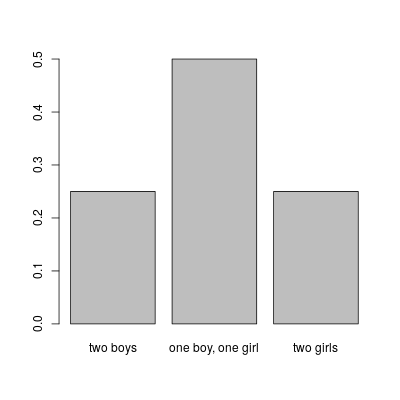
\includegraphics[scale=.45]{./diagrams/boys.png}
\end{figure}
\end{frame}

\begin{frame}
  \frametitle{Discrete Probability Distribution Graphs II}
  \beispiel{Immigrant Languages}\label{ex:ahchoiyu} Here is the
  probability distribution for a randomly selected ``Vancouverite''
  (Greater Vancouver) to speak a certain immigrant language at home.

\vspace{-.5in}

\begin{figure}[h]
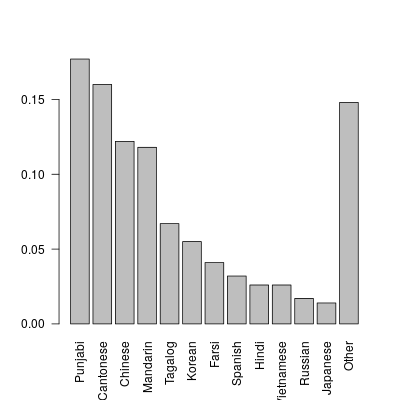
\includegraphics[scale=.5]{./diagrams/vanlang.png}
\end{figure}
\end{frame}

\begin{frame}
  \frametitle{Mean and Variance Formulas}
There is a sense in which a probability distribution together with its
associated random variable correspond to a population and the property
which the random variable picks out. In this spirit, let us define a
mean and a variance for a probability distribution.
\begin{equation}
  \label{eq:noohahfa}
  \mu=\sum{}X\cdot{}P(X)
\end{equation}
\begin{equation}
  \label{eq:axiengeb}
  \sigma^{2}=\sum(X-\mu)^{2}\cdot{}P(X)
\end{equation}
\begin{equation}
  \label{eq:teeneilu}
  \sigma^{2}=\sum(X^{2}\cdot{}P(X))-\mu^{2}
\end{equation}
\begin{equation}
  \label{eq:iifiekai}
  \sigma=\sqrt{\sum(X^{2}\cdot{}P(X))-\mu^{2}}
\end{equation}
\end{frame}

\begin{frame}
  \frametitle{Die Roll Example}
\beispiel{Fair Die Roll}\label{ex:reinooth} Think of rolling a fair die
many times. The probability distribution is uniform. The mean is
\begin{equation}
  \label{eq:isiamaih}
   \mu=\sum{}X\cdot{}P(X)=1\cdot{}\frac{1}{6}+2\cdot{}\frac{1}{6}+3\cdot{}\frac{1}{6}+4\cdot{}\frac{1}{6}+5\cdot{}\frac{1}{6}+6\cdot{}\frac{1}{6}=3.5\notag
\end{equation}
We also call this number the \alert{expectation} $EX$ of the random
variable $X$. Although you would never expect a die roll to result in
``3.5,'' you would expect the mean of many die rolls to be close to
this number. The expected number of boys for one birth is $EX=0.5$.
\end{frame}

\begin{frame}
  \frametitle{The Binomial Probability Distribution}
A \alert{binomial probability distribution} results from a procedure
that meets the following requirements.
\begin{enumerate}
\item The procedure has a fixed number of trials.
\item The trials must be independent.
\item The outcomes of a trial are binary, i.e.\ there are only two
  possible outcomes.
\item The probability of the two outcomes remains constant.
\end{enumerate}
The number of trials is usually labeled $n$, the two outcomes are
called \alert{success} and \alert{failure}, and their probabilities on
one trial are $p$ and $1-p$. The random variable keeps track of the
number of successes. If, for example, there are 10 trials, then
$P(X=4)$ is the probability of 4 successes out of 10. The number of
successes is often labeled $x$, and we are usually interested in
$P(X=x)$.
\end{frame}

\begin{frame}
  \frametitle{Calvin on the Binomial Distribution}
\begin{figure}[h]
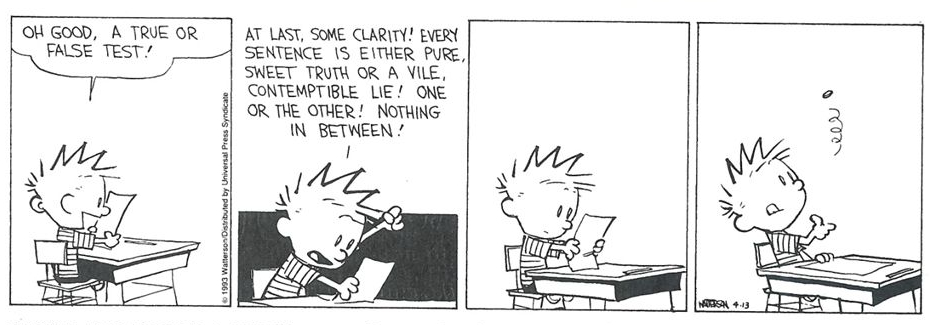
\includegraphics[scale=.43]{./diagrams/calvin_hobbes_binomial_edited.jpg}
\end{figure}
\end{frame}

\begin{frame}
  \frametitle{The Binomial Probability Formula}
If $n,p,x$ are as described on the previous slide, then
\begin{equation}
  \label{eq:pheehael}
  % P(X=x)={n\choose{}x}\cdot{}p^{x}\cdot(1-p)^{n-x}
  P(X=x)=\binom{n}{x}\cdot{}p^{x}\cdot(1-p)^{n-x}
\end{equation}
\end{frame}

\begin{frame}
  \frametitle{The Binomial Distribution and R}
Here are some R commands that help with the binomial distribution.

\bigskip

(1) Find the probability for 7 successes on 12 trials when the
probability of success is 40\% ($x=7,n=12,p=0.4$):
\begin{alltt}
  dbinom(7,12,0.4)\newline
  0.1009024
\end{alltt}
\end{frame}

\begin{frame}
  \frametitle{The Binomial Distribution and R}
(2) Do the same for $x=0,1,2,3,4,5$ and $n=5,p=0.40$:
\begin{alltt}
  dbinom(0:5,5,0.4)\newline
  0.07776 0.25920 0.34560 0.23040 0.07680 0.01024
\end{alltt}
(3) You can plot this distribution using (notice how skewed the
distribution is because of $p=0.40$):
\begin{alltt}
  x<-dbinom(0:5,5,0.4)\newline
  barplot(x)
\end{alltt}
\end{frame}

\begin{frame}
  \frametitle{The Binomial Distribution and R}
(4) Often, you want to add the probabilities for a range of $x$. For
example, what is the probability of having strictly fewer than 3
successes on 5 trials with $p=0.7$?
\begin{alltt}
  pbinom(2,5,0.4)\newline
  0.68256
\end{alltt}
(5) You can list these probabilities as follows:
\begin{alltt}
  pbinom(0:5,5,0.4)\newline
  0.07776 0.33696 0.68256 0.91296 0.98976 1.00000
\end{alltt}
\end{frame}

\begin{frame}
  \frametitle{The Binomial Distribution and R}
(6) You can simulate a binomial distribution using \texttt{rbinom}.
Conduct 100 experiments where you perform 12 trials with a success
probability $p=0.4$. Here are the results (number of successes $x$)
with a barplot:
\begin{alltt}
x<-rbinom(100,12,0.4)\newline
5 5 5 4 8 6 4 7 7 3 4 2 8 4 6 6 6 6 4 4 3 3 3 4 4 5 8 5 4 7 7 5 6 4 6 3 5
6 4 4 7 5 5 4 7 6 5 3 5 8 5 5 5 6 6 6 5 6 5 3 5 4 4 6 5 4 5 6 6 6 3 5 2 6
7 6 6 2 3 5 3 4 5 3 5 5 5 4 6 1 6 3 3 2 6 4 4 3 4 4\newline
barplot(table(x))
\end{alltt}
\end{frame}

\begin{frame}
  \frametitle{Exercises for the Binomial Distribution I}
  {\ubung} If you randomly guess on a multiple choice test with four
  possible answers, what is your probability of getting strictly more than 50\%
  of questions right when there are six questions?
\end{frame}

\begin{frame}
  \frametitle{Exercises for the Binomial Distribution II}
  {\ubung} The incidence of blue eyes in the population is 12\%. In a room
  with 20 randomly selected people, what is the probability of having
  three or more people with blue eyes? What is the probability of
  having strictly fewer than five people with blue eyes? 
  \begin{quote}
    Strictly speaking, the binomial probabilities are only approximate
    because the selection happens without replacement. If the
    population is large from which the sample is drawn, then you are
    allowed to ignore this.
  \end{quote}
\end{frame}

\begin{frame}
  \frametitle{Exercises for the Binomial Distribution III}
  {\ubung} Here is the distribution of blood types in Canada.

\bigskip

  \begin{tabular}{|l|r|r|r|r|}\hline
         & O     & A     & B     & AB    \\ \hline
Positive & 0.390 & 0.360 & 0.076 & 0.025 \\ \hline
Negative & 0.070 & 0.060 & 0.014 & 0.005 \\ \hline
  \end{tabular}

\bigskip

(a) What is the probability of being rhesus factor positive for
someone of blood type ``A''?

\medskip

(b) If you meet four randomly selected Canadians, what is the
probability that two of them are ``O'' positive?

\medskip

(c) In a room with twelve randomly selected Canadians, what is the
probability that there are strictly fewer than three people with
blood type ``B''?
\end{frame}

\begin{frame}
  \frametitle{Exercises for the Binomial Distribution IV}
  {\ubung} 80.5\% of US flights arrive on time. For twelve randomly
  selected flights, what is the probability that exactly ten of them
  are on time? What is the probability that between two and four of
  them are not on time?
\end{frame}

\begin{frame}
  \frametitle{Mean and Variance for the Binomial Distribution}
There are formulas for the mean and variance of the binomial
distribution. Especially the formula for the mean makes immediate
sense:
\begin{block}{Formulas}
  \begin{tabular}{llcr}
  mean& $\mu$&$=$&$np$ \\ 
  variance& $\sigma^{2}$&$=$&$npq$ \\
  standard deviation& $\sigma$&$=$&$\sqrt{npq}$
  \end{tabular}
\end{block}
It is a useful rule of thumb to remember that it is unlikely ($<5\%$)
that $x$ is outside of the interval from $\mu-2\sigma$ to
$\mu+2\sigma$.
\end{frame}

\begin{frame}
  \frametitle{Exercises for the Binomial Distribution V}
  {\ubung} What is the rule-of-thumb 95\% interval for the following
  binomial procedures:
  \begin{enumerate}
\item<1-> flipping a fair coin 15 times
\item<2-> answering 60 multiple choice questions with four possible
  answers for each question, where the probability of getting the right answer is 80\%
\item<3-> randomly answering 60 multiple choice questions with four
  possible answers for each question
\item<4-> The number of ``O'' positive blood types in a crowd of 100 Canadians.
  \end{enumerate}
\end{frame}

\begin{frame}
  \frametitle{Poisson Distribution}
The \alert{Poisson Distribution} is another discrete probability
distribution. It applies to occurrences of some event over a specified
interval, such as time or distance. The probability of the event
occurring $x$ times over an interval is given by
\begin{equation}
  \label{eq:zaengeit}
  P(X=x)=\frac{\lambda^{x}\cdot{}e^{-\lambda}}{x!}
\end{equation}
where $e$ is Euler's number ($\approx{}2.71828$) and $\lambda$ is the mean
number of occurrences over the interval.
\end{frame}

\begin{frame}
  \frametitle{Poisson Distribution Example}
\beispiel{Earthquakes} The mean number of annual major earthquakes
in the world is 0.93. Calculate the probability of $x$ earthquakes
happening in one year.

\medskip

\begin{tabular}{|r|r|r|}\hline
  Number of Earthquakes & Poisson Distribution & Actual Figure \\ \hline 
  0                     & 0.3946               & 47 out of 100 \\ \hline
  1                     & 0.3669               & 31 out of 100 \\ \hline
  2                     & 0.1706               & 13 out of 100 \\ \hline
  3                     & 0.0529               & 5 out of 100  \\ \hline
  4                     & 0.0123               & 2 out of 100  \\ \hline
  5                     & 0.0029               & 0 out of 100  \\ \hline
  6                     & 0.0004               & 1 out of 100  \\ \hline
  7                     & 0+                   & 1 out of 100  \\ \hline
\end{tabular}
\end{frame}

% \begin{frame}
%   \frametitle{Poisson Distribution in R}
% In R Statistics, you use the following command to find the poisson distribution. 
% \begin{alltt}
%   dpois(2,lambda=0.93)
% \end{alltt}
% for the probability of $x=2$ with $\lambda=0.93$.
% \begin{alltt}
%   ppois(16,lambda=12)
% \end{alltt}
% for the probability of $x$ being \alert{16 or less} with $\lambda=12$.
% \end{frame}

\begin{frame}
  \frametitle{Summary}
The binomial and Poisson distributions are discrete probability
distributions. The formulas are as follows.
\begin{equation}
  \label{eq:hiechoib}
  \mbox{\textbf{[binomial] }}P(X=x)=\binom{n}{x}\cdot{}p^{x}\cdot(1-p)^{n-x}\mbox{ for }(x,n,p)\notag
\end{equation}
\begin{equation}
  \label{eq:iechahve}
  \mbox{\textbf{[Poisson] }}P(X=x)=\frac{\lambda^{x}\cdot{}e^{-\lambda}}{x!}\mbox{ for }(x,\lambda)\notag
\end{equation}
Use the following functions in R Statistics.
\begin{itemize}
\item $P(X=x)=$\texttt{dbinom(x,n,p)} for binomial, not cumulative.
\item $P(X\leq{}x)=$\texttt{pbinom(x,n,p)} for binomial, cumulative.
\item $P(X=x)=$\texttt{dpois(x,$\lambda$)} for Poisson, not cumulative.
\item $P(X\leq{}x)=$\texttt{ppois(x,$\lambda$)} for Poisson, cumulative.
\end{itemize}
\end{frame}

\begin{frame}
  \frametitle{Exercise I}
  {\ubung} A river causes 15 floods in 100 years in the long run. The
  floods occur independently of each other. What is the probability
  for 3 or more floods to occur in the next 10 years?
\end{frame}

\begin{frame}
  \frametitle{Exercise II}
  {\ubung} Mars Inc. tells us that 20\% of M\&Ms are orange. A bag
  contains 42 M\&Ms. What is the probability of a bag containing
  between 7 and 9 orange M\&Ms?
\end{frame}

\begin{frame}
  \frametitle{Exercise III}
  {\ubung} Over the last 100 million years, 600 climate-changing
  meteors have hit the Earth. What is the probability of one or more
  climate-changing meteors hitting the Earth in the next 100 years?
\end{frame}

\begin{frame}
  \frametitle{Exercise IV}
  {\ubung} The average number of goals in a World Cup soccer match is
  approximately 2.5. What is the probability that a match ends
  scoreless? What is the probability that strictly more than 3 goals
  are scored in a match?
\end{frame}

\begin{frame}
  \frametitle{Exercise V}
  {\ubung} Twenty people each roll a die. What is the probability that
  five of them roll either a one or a two?
\end{frame}

\begin{frame}
  \frametitle{Exercise VI} {\ubung} You get 15 phone calls every day.
  They happen independently of the time of day. What is the
  probability of getting a phone call in the next 25 minutes?
\end{frame}

\begin{frame}
  \frametitle{Approximating Binomial Probabilities I}
Here is the formula for a \alert{binomial} setup with $n$ trials (for example,
$n=2$ coin tosses), probability of success $p$ (for example, $p=0.5$ for the
probability of heads), and $x$ number of successes,
\begin{equation}
  \label{eq:iedohdah}
  P(X=x)=\frac{n!}{(n-x)!x!}p^{x}(1-p)^{n-x}
\end{equation}
where $0!=1$ and $(n+1)!=n!(n+1)$, for example
$4!=1\cdot{}2\cdot{}3\cdot{}4$ (say ``four factorial''). $X$ is a
\alert{random variable}, the number that the random process spits out.
\end{frame}

\begin{frame}
  \frametitle{Approximating Binomial Probabilities II}
Here are the binomial probabilities for $n=6$. One way to
conceptualize these numbers is by looking at Pascal's Triangle (next
slide). 
  \begin{figure}[h]
    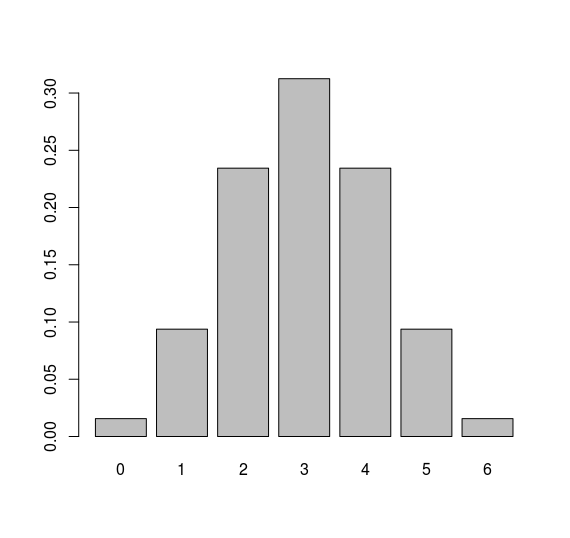
\includegraphics[scale=.5]{./diagrams/binomial1.png}
  \end{figure}
\end{frame}

\begin{frame}
  \frametitle{Pascal's Triangle}
\begin{tikzpicture}
\foreach \n in {0,...,7} {
  \foreach \k in {0,...,\n} {
    \node at (\k-\n/2,-\n) {$\binomialCoefficient{\n}{\k}$};
  }
}
\end{tikzpicture}
\end{frame}

\begin{frame}
  \frametitle{Pascal's Triangle}
\begin{tikzpicture}
\foreach \n in {0,...,7} {
  \foreach \k in {0,...,\n} {
    \node at (\k-\n/2,-\n) {$\binom{\n}{\k}$};
  }
}
\end{tikzpicture}
\end{frame}

\begin{frame}
  \frametitle{Approximating Binomial Probabilities III}
Binomial probabilities are difficult to calculate for high numbers. We
approximate the binomial distribution with the \alert{normal distribution}.
Compare the binomial distribution for $n=10$ with the normal
distribution.
  \begin{figure}[h]
    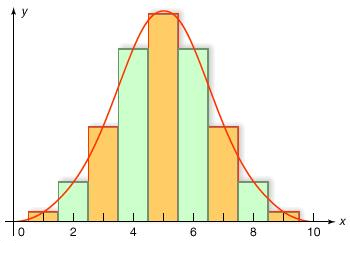
\includegraphics[scale=.5]{./diagrams/binnorm1_ed.jpg}
  \end{figure}
\end{frame}

\begin{frame}
  \frametitle{Normal Distribution}
  The normal probabilities distribution is a \alert{continuous}
  probabilities distribution. There is not just one normal
  distribution. There are infinitely many, characterized by their
  \alert{mean $\mu$} and their \alert{standard deviation $\sigma$}.
  The formula for the normal distribution is
  \begin{equation}
    \label{eq:aitoolah}
    f(x)=\frac{1}{\sigma\sqrt{2\pi}}e^{-(x-\mu)^{2}/(2\sigma^{2})}
  \end{equation}
  \begin{figure}[h]
    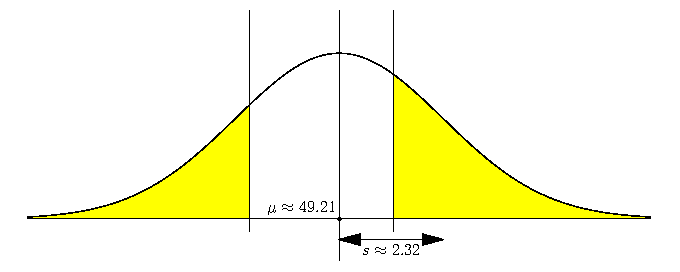
\includegraphics[scale=.4]{./diagrams/qfour.png}
  \end{figure}
\end{frame}

\begin{frame}
  \frametitle{Z Scores}
  To calculate the area under the curve, we carry around a piece of
  paper with all the values for the \alert{standard normal
    distribution} and then convert to the normal distribution with the
  relevant $\mu$ and $\sigma$. The value for the normal distribution
  is called the \alert{$x$-score} and its associate value for the
  standard normal distribution is called the \alert{$z$-score}. Travel
  back and forth using the following formula,
  \begin{equation}
    \label{eq:uotoogoo}
    z=\frac{x-\mu}{\sigma}
  \end{equation}
\end{frame}

\begin{frame}
  \frametitle{Normal Distribution Example Question}
  \beispiel{Men's Heights} The height of adult men is normally
  distributed with mean $\mu=69.5$ inches and standard deviation
  $\sigma=2.4$ inches. What percentage of the adult male population is
  taller than six feet (72 inches)? 
\end{frame}

\begin{frame}
  \frametitle{Normal Distribution Example Answer}
  Find the $z$-score, using the formula
  \begin{equation}
    \label{eq:igutheib}
    z=\frac{x-\mu}{\sigma}=\frac{72-69.5}{2.4}\approx{}1.04
  \end{equation}
  Use your $z$-score table to find the corresponding
  \alert{$p$-value}, which is the area to the left of the $z$-score
  for the standard normal distribution. In this case the $p$-value is
  $0.8508$. This represents the percentage of the male population that
  is \emph{shorter} than 72 inches. The answer to our question is
  therefore, 14.92\% of men are taller than six feet.
\end{frame}

\begin{frame}
  \frametitle{Normal Distribution Exercises I}
{\ubung} Find the area under the curve for the following sets of
$z$-scores. 
\begin{equation}
  \label{eq:deapheph}
\{z|z\leq{}-1.72\}  
\end{equation}
\begin{equation}
  \label{eq:taedaiga}
\{z|1.96<{}z\}  
\end{equation}
\begin{equation}
  \label{eq:ahraefis}
\{z|-1.55\leq{}z\leq{}-0.81\}
\end{equation}
\end{frame}

\begin{frame}
  \frametitle{Normal Distribution Exercises II}
{\ubung} Find the area under the curve for the
following sets of $x$-scores. 
\begin{equation}
  \label{eq:aequaixe}
\{x|x\leq{}83\},\mu=100,\sigma=15
\end{equation}
\begin{equation}
  \label{eq:oocohdau}
\{x|0.44<x\},\mu=0.5,\sigma=0.2  
\end{equation}
\begin{equation}
  \label{eq:aethohph}
\{x|800\leq{}x\leq{}1200\},\mu=911,\sigma=121
\end{equation}
\end{frame}

\begin{frame}
  \frametitle{Normal Distribution Exercises III}
{\ubung} The time it takes a student to solve a particular math problem is
normally distributed with $\mu=3$ minutes and $27$ seconds and a
standard deviation of $\sigma=59$ seconds. How many students finish
the math problem between 3 and 4 minutes?
\end{frame}

\begin{frame}
  \frametitle{Normal Distribution Exercises IV}
  {\ubung} Scores on a certain intelligence test for children between
  ages 13 and 15 years are approximately normally distributed with
  $\mu=106$ and $\sigma=15$.
  \begin{enumerate}
  \item What proportion of children aged 13 to 15 years old have
    scores on this test above 88?
  \item Enter the score which marks the lowest 30 percent of the
    distribution.
  \item Enter the score which marks the highest 15 percent of the
    distribution.
  \end{enumerate}
When you want to find an $x$-score given a $p$-value, you need to use
your table in reverse and then find the $x$-score given the $z$-score
from the table by using the formula
\begin{equation}
  \label{eq:aedecaba}
  x=z\cdot\sigma+\mu
\end{equation}
\end{frame}

\begin{frame}
  \frametitle{Approximating Binomial Probabilities Example I}
  For large numbers, even high-powered computers cannot calculate the
  binomial probabilities. We use the normal distribution to
  approximate the binomial distribution. 

\bigskip

  \beispiel{Die Rolls} If you roll a die 600 times, what is the
  probability of rolling a six fewer than 80 times? 

\bigskip

  It would take very long to calculate this probability using the
  binomial distribution formula! We use the normal distribution with
  $\mu=np$ and $\sigma=\sqrt{np(1-p)}$ instead. 

\bigskip

  Conventionally, it is only acceptable to approximate the binomial
  distribution by the normal distribution if $np\geq{}5$ and
  $nq\geq{}5$. Otherwise, the binomial and the normal distribution are
  too far apart to provide a useful approximation.
\end{frame}

\begin{frame}
  \frametitle{Approximating Binomial Probabilities Example II}
  We need to make a \alert{continuity correction} and ask ourselves,
  what is the probability for the $x$-score to be 79.5 or less for
  this normal distribution?
  \begin{equation}
    \label{eq:oolojuth}
    z=\frac{x-\mu}{\sigma}=\frac{79.5-100}{9.1287}\approx{}-2.25
  \end{equation}
  The corresponding $p$-value is 0.0122. There is only a 1.22\%
  probability that you will roll fewer than 80 sixes in 600 rolls.
\end{frame}

\begin{frame}
  \frametitle{Continuity Correction}
  % Continuity correction means that when we approximate a whole number
  % $m$ using the continuous normal distribution, we use the interval
  % $[m-0.5,m+0.5]$ to represent this whole number. ``Fewer than 80,''
  % for example, is translated for the approximation as ``less than
  % 79.5.'' ``Fewer than or equal to 80'' is translated as ``less than
  % 80.5.''
  \begin{figure}[h]
    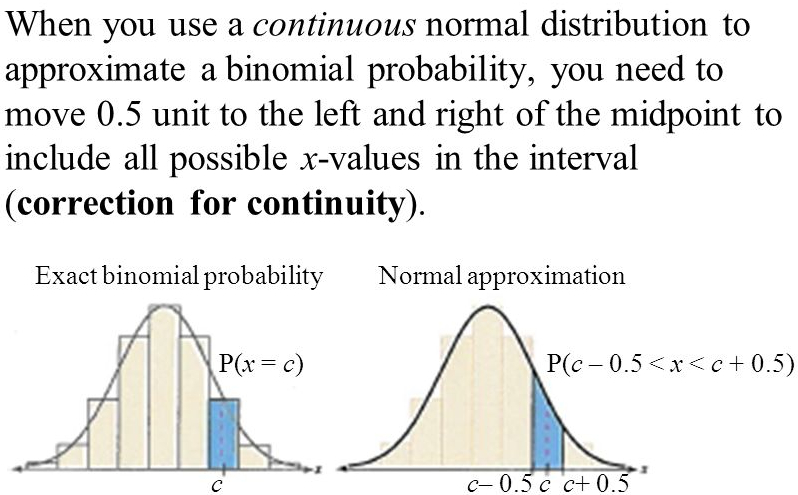
\includegraphics[scale=.5]{./diagrams/contcorr_ed1.jpg}
  \end{figure}
\end{frame}

\begin{frame}
  \frametitle{Binomial Approximation Exercise}
{\ubung} 29\% of a country's population is blue-eyed. What is the
probability that a random sample of 1,000 persons contains between 200
and 300 blue-eyed persons? Approximate the binomial distribution by
the normal distribution. Calculate $\mu=np$ and
$\sigma=\sqrt{np(1-p)}$ for this normal distribution after checking
the conditions $np\geq{}5,n(1-p)\geq{}5$. Then calculate the
$z$-scores for the $x$-scores $x=199.5$ and $x=300.5$. Lastly,
determine the area under the curve between these $z$-scores. Provide a
complete sentence to answer the question.
\end{frame}

\begin{frame}
  \frametitle{Word Problems}
  {\ubung} The national mortality rate for a particular type of heart
  surgery is 12\%, so you would expect six deaths per 50 operations.
  You are a health administrator, and one of your doctors has had
  eleven deaths in 72 operations. Should you fire her? What is the
  probability that an average surgeon (whose mortality rate is the
  national average) will have eleven or more deaths in 72 operations?
\end{frame}

\begin{frame}
  \frametitle{Word Problems}
  {\ubung} You desperately need a person with blood type AB (incidence
  in Canada: 3\%). If there are 49 people in the room, what is the
  probability that at least one of them is AB?
\end{frame}

\begin{frame}
  \frametitle{Word Problems}
  {\ubung} Based on observed males using public restrooms, 85\% of
  adult males wash their hands in a public restroom (based on data
  from the American Society for Microbiology and the American Cleaning
  Institute). In a survey of 523 adult males, 518 reported that they
  wash their hands in a public restroom. Assuming that the 85\%
  observed rate is correct, find the probability that among 523
  randomly selected adult males, 518 or more wash their hands in a
  public restroom. What do you conclude?
\end{frame}

\begin{frame}
  \frametitle{Word Problems}
  {\ubung} In a survey of 1002 people, 701 said that they voted in a
  recent presidential election (based on data from ICR Research
  Group). Voting records show that 61\% of eligible voters actually
  did vote. Given that 61\% of eligible voters actually did vote, find
  the probability that among 1002 randomly selected eligible voters,
  at least 701 actually did vote. What does the result suggest?
\end{frame}

\begin{frame}
  \frametitle{Word Problems}
  {\ubung} In a study of 420,095 cell phone users in Denmark, it was
  found that 135 developed cancer of the brain or nervous system.
  Assuming that the use of cell phones has no effect on developing
  such cancers, there is a 0.000340 probability of a person developing
  cancer of the brain or nervous system. We therefore expect about 143
  cases of such cancers in a group of 420,095 randomly selected
  people. Estimate the probability of 135 or fewer cases of such
  cancers in a group of 420,095 people. What do these results suggest
  about media reports that cell phones cause cancer of the brain or
  nervous system?
\end{frame}

\begin{frame}
  \frametitle{Word Problems}
  {\ubung} Based on a recent Harris Interactive survey, 20\% of adults
  in the United States smoke. In a survey of 50 statistics students,
  it is found that six of them smoke. Find the probability that should
  be used for determining whether the 20\% rate is correct for
  statistics students. What do you conclude?
\end{frame}

\begin{frame}
  \frametitle{Word Problems}
  {\ubung} Online TV In a Comcast survey of 1000 adults, 17\% said
  that they watch prime-time TV online. If we assume that 20\% of
  adults watch prime-time TV online, find the probability that should
  be used to determine whether the 20\% rate is correct or whether it
  should be lower than 20\%? What do you conclude?
\end{frame}

\begin{frame}
  \frametitle{Word Problems}
  {\ubung} Internet Access Of U.S. households, 67\% have Internet
  access (based on data from the Census Bureau). In a random sample of
  250 households, 70\% are found to have Internet access. Find the
  probability that should be used to determine whether the 67\% rate
  is too low. What do you conclude?
\end{frame}

% \begin{frame}
%   \frametitle{Word Problems II}
%   \begin{figure}[h]
%     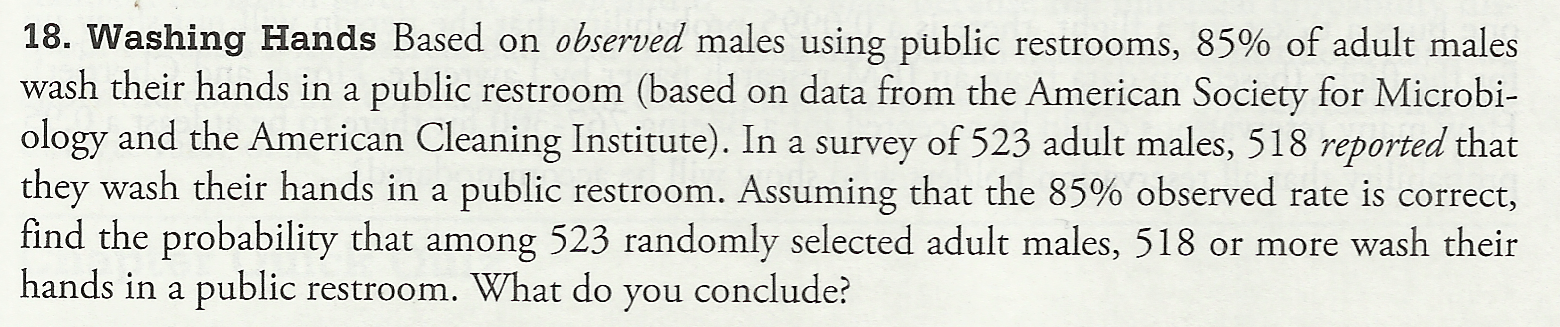
\includegraphics[scale=.7]{./diagrams/triola1.png}
%   \end{figure}
%   \begin{figure}[h]
%     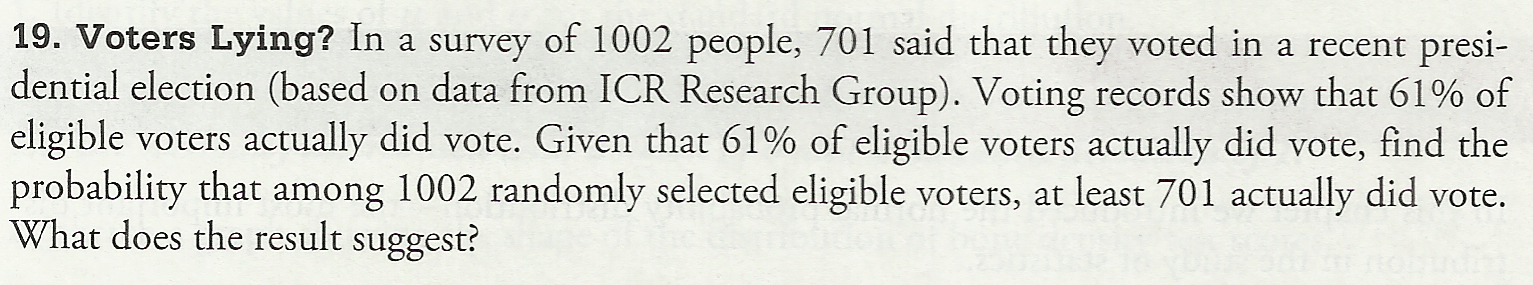
\includegraphics[scale=.7]{./diagrams/triola2.png}
%   \end{figure}
%   \begin{figure}[h]
%     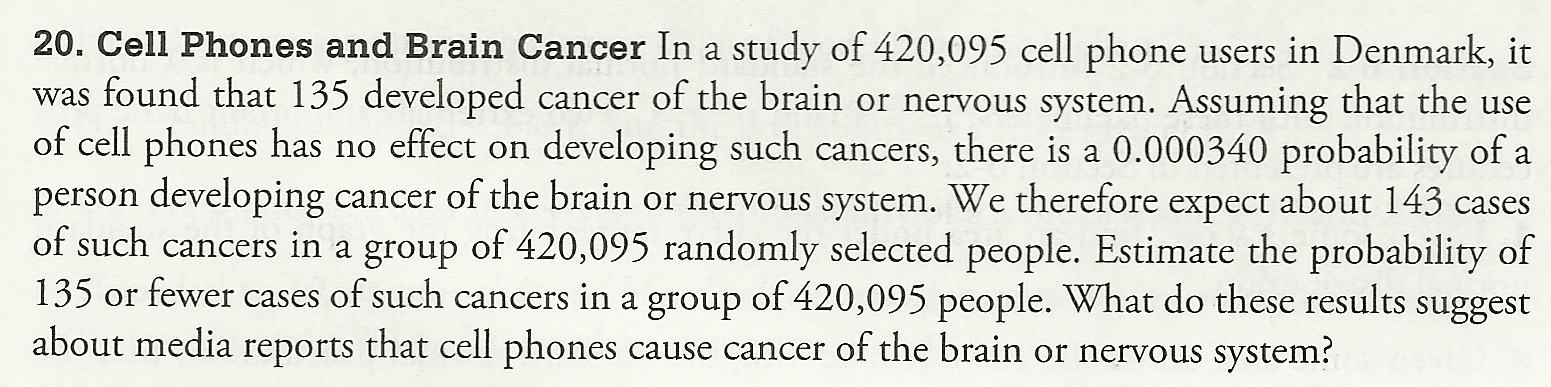
\includegraphics[scale=.7]{./diagrams/triola3.png}
%   \end{figure}
% \end{frame}

% \begin{frame}
%   \frametitle{Word Problems III}
%   \begin{figure}[h]
%     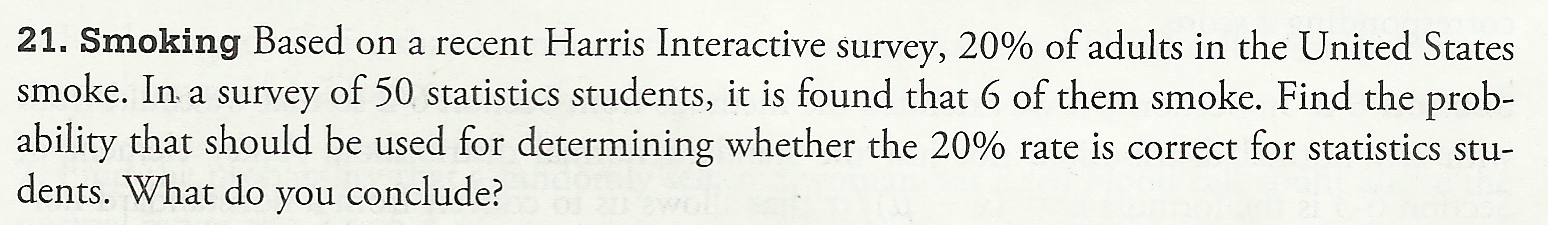
\includegraphics[scale=.7]{./diagrams/triola4.png}
%   \end{figure}
%   \begin{figure}[h]
%     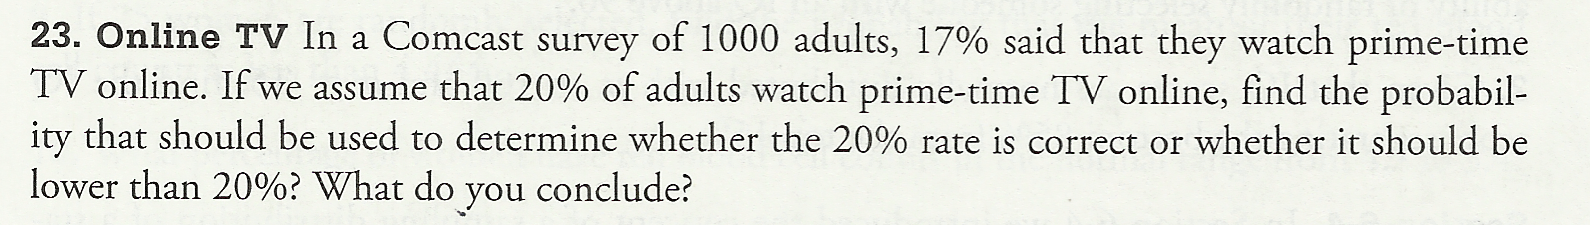
\includegraphics[scale=.7]{./diagrams/triola5.png}
%   \end{figure}
%   \begin{figure}[h]
%     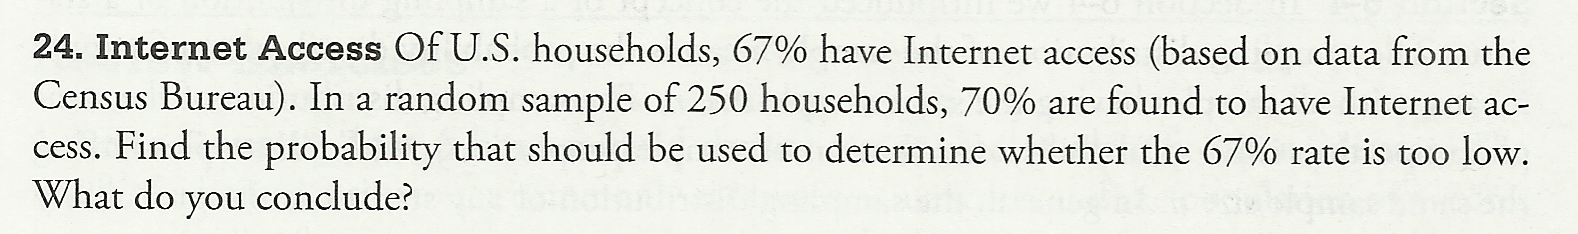
\includegraphics[scale=.7]{./diagrams/triola6.png}
%   \end{figure}
% \end{frame}

\begin{frame}
  \frametitle{Using Poisson to Approximate Binomial}
% http://courses.wcupa.edu/rbove/Berenson/10th%20ed%20CD-ROM%20topics/section5_6.pdf
  Situations in which $n$ is large and $p$ is very small:
  \begin{enumerate}
  \item I cannot use the binomial formula because my calculator cannot
    handle $n!$.
  \item I cannot use the normal distribution to approximate the
    binomial distribution because $n\cdot{}p<5$.
  \end{enumerate}
  The Poisson distribution can be used to approximate the binomial
  distribution. The larger the $n$ and the smaller the $p$, the better
  the approximation. We use the Poisson distribution for which
  $\lambda=np$.
\end{frame}

\begin{frame}
  \frametitle{Using Poisson to Approximate Binomial}
    \begin{figure}[h]
    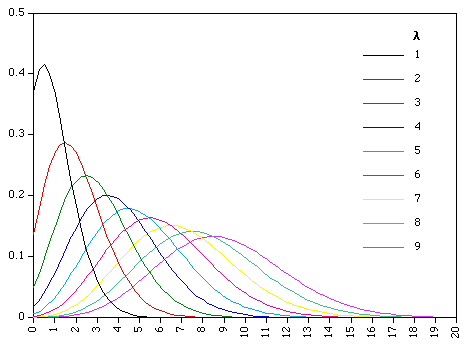
\includegraphics[scale=.62]{./diagrams/poisdist.png}
  \end{figure}
\end{frame}

\begin{frame}
  \frametitle{Using Poisson to Approximate Binomial}
  \beispiel{Manufacturing Tires} Suppose 8\% of the tires manufactured
  at a particular plant are defective. Estimate the probability of obtaining
  exactly one defective tire from a sample of twenty.
  \begin{equation}
    \label{eq:eikaiche}
    P(X=1)^{\mbox{\tiny binomial}}={20\choose{}1}0.08^{1}\cdot0.92^{19}=0.3281623
  \end{equation}
  is approximately
  \begin{equation}
    \label{eq:aihuroot}
    P(X=1)^{\mbox{\tiny poisson}}=\frac{e^{-1.6}(1.6)^{1}}{1!}=0.3230344
  \end{equation}
\end{frame}

\begin{frame}
  \frametitle{Using Poisson to Approximate Binomial Exercises}
  {\ubung} Based upon past experience, 1\% of the telephone bills
  mailed to households are incorrect. If a sample of twenty bills is
  selected, find the probability that at least one bill will be
  incorrect. Do this using two probability distributions (the binomial
  and the Poisson) and compare your results.
\end{frame}

\begin{frame}
  \frametitle{Using Poisson to Approximate Binomial Exercises}
  {\ubung} A computer manufacturing company conducts acceptance
  sampling for incoming computer chips. After receiving a huge
  shipment of computer chips, the company randomly selects 800 chips.
  If three or fewer nonconforming chips are found, the entire lot is
  accepted without inspecting the remaining chips in the lot. If four
  or more chips are nonconforming, every chip in the entire lot is
  carefully inspected at the supplier's expense. Assume that the true
  proportion of nonconforming computer chips being supplied is 0.001.
  What is the probability the lot will be accepted?
\end{frame}

\begin{frame}
  \frametitle{Using Poisson to Approximate Binomial Exercises}
  {\ubung} Last month your company sold ten thousand new watches. Past
experience indicates that the probability that a new watch
will  need  repair  during  its  warranty  period  is  0.002.

Compute the probability that:
\begin{enumerate}
\item zero watches will need warranty work
\item no more than 5 watches will need warranty work
\item no more than 10 watches will need warranty work
\item no more than 20 watches will need warranty work
\end{enumerate}
\end{frame}

\begin{frame}
  \frametitle{End of Lesson}
Next Lesson: Central Limit Theorem
\end{frame}

\end{document}
